% =====================================================================
%  Drone Detection Using YOLO11
%  B.Tech Semester 6 Project Report
%  Indian Institute of Information Technology, Guwahati
% =====================================================================
\documentclass[12pt,a4paper]{report}

\usepackage[utf8]{inputenc}
\usepackage[T1]{fontenc}
\usepackage{lmodern}
\usepackage[margin=1in]{geometry}
\usepackage{graphicx}
\usepackage{booktabs}
\usepackage{caption}
\usepackage{subcaption}
\usepackage{amsmath}
\usepackage{float}
\usepackage{enumitem}
\usepackage{fancyhdr}
\usepackage{titlesec}
\usepackage{setspace}
\usepackage{parskip}
\usepackage{url}
\usepackage[hidelinks]{hyperref}
\usepackage{tikz}
\usetikzlibrary{shapes.geometric, arrows.meta, positioning, calc}

% ----- Page style -----
\pagestyle{fancy}
\fancyhf{}
\fancyhead[L]{\small\itshape Drone Detection Using YOLO11}
\fancyhead[R]{\small\itshape IIITG, B.Tech Project}
\fancyfoot[C]{\thepage}
\renewcommand{\headrulewidth}{0.4pt}

\titleformat{\chapter}[display]
  {\normalfont\Large\bfseries\centering}
  {\MakeUppercase{\chaptertitlename}\ \thechapter}{14pt}{\Large\MakeUppercase}
\titleformat{\section}{\large\bfseries}{\thesection}{1em}{}
\titleformat{\subsection}{\normalsize\bfseries}{\thesubsection}{1em}{}

\onehalfspacing

\begin{document}

% =====================================================================
%  PAGE 1 — TITLE PAGE  (senior-style layout)
% =====================================================================
\begin{titlepage}
\begin{center}

\vspace*{1.5cm}

{\LARGE\bfseries Drone Detection Using YOLO11}\\[2.5cm]


\includegraphics[width=0.42\textwidth,keepaspectratio]{graphs/iiitg_logo.png}\\[2.0cm]

{\large\bfseries Gajendra Gangwar}\\[0.2cm]
{\large\bfseries Roll No.: 2301081}\\[0.5cm]

{\normalsize Advisor: \textbf{Dr.\ Rakesh Matam}}\\[0.4cm]

{\normalsize Department of Computer Science and Engineering}\\
{\normalsize Indian Institute of Information Technology Guwahati}

\vfill

\end{center}

\noindent
{\normalsize IIIT Guwahati}
\hfill
{\normalsize April 2026}

\end{titlepage}

% =====================================================================
%  PAGE 2 — DECLARATION
% =====================================================================
\thispagestyle{plain}
\begin{center}
{\Large\bfseries DECLARATION}
\end{center}
\vspace{0.8cm}

I declare that this project report titled \textbf{``Drone Detection Using
YOLO11''} is the result of my own work, carried out under the guidance of
Dr.~Rakesh Matam, Department of Computer Science and Engineering, IIIT Guwahati.
The dataset used in this work was originally prepared by Madhubani Basu, and has been re-used here only so that the two approaches can be
compared on the same data. To the best of my knowledge, this work has not been
submitted anywhere else for the award of any degree, and all sources I have
referred to have been duly cited.

\vspace{2cm}

\noindent
\begin{flushleft}
\textbf{Gajendra Gangwar}\\
Roll No.: 2301081\\
B.Tech, Computer Science and Engineering\\
Indian Institute of Information Technology, Guwahati
\end{flushleft}

\newpage

% =====================================================================
%  PAGE 3 — ACKNOWLEDGEMENT
% =====================================================================
\thispagestyle{plain}
\begin{center}
{\Large\bfseries ACKNOWLEDGEMENT}
\end{center}
\vspace{0.8cm}

I would like to thank my advisor \textbf{Dr.~Rakesh Matam} for his constant
guidance throughout this project. His suggestions on how to plan the training
and how to evaluate the model properly were very helpful. I would also like to
thank \textbf{Madhubani Basu}, whose earlier work on the same problem
gave me the dataset and a clear starting point, and who patiently answered my
questions while I was getting familiar with it.

\vspace{1.5cm}
\noindent
\hfill \textbf{Gajendra Gangwar}\\
\hfill Roll No.\ 2301081\\
\hfill B.Tech CSE, Semester~6\\
\hfill IIIT Guwahati

\newpage

% =====================================================================
%  PAGE 4 — ABSTRACT
% =====================================================================
\thispagestyle{plain}
\begin{center}
{\Large\bfseries ABSTRACT}
\end{center}
\vspace{0.4cm}

Drones are now easily available to anyone, and while they are useful for many
good purposes, their misuse near airports, military areas, and public events has
become a real concern. A reliable visual drone-detection system is therefore
needed.

This project builds on the earlier in-house work by Madhubani Basu, in
which the drone/non-drone dataset was prepared and a YOLOv9 + EfficientNet-B3
model was trained. In the present work, the same dataset is re-used and a
different, more recent model -- \textbf{YOLO11-nano} -- is trained on it, so that
the two pipelines can be compared fairly.

Six modern detectors (YOLOv9, YOLO11, RT-DETR, YOLO26, NSSRD, ED-Net) were first studied, and YOLO11-nano was selected because it offers a good balance between accuracy on small objects and the limited compute resources available. The model was trained in \textbf{two phases}: epochs 1\,--\,200 from
scratch and epochs 201\,--\,500 resumed from the Phase~1 checkpoint.

The trained model was then evaluated in three ways: (i) on the full validation
set, (ii) on a \textbf{distance-wise split} (close-range, mid-range, long-range,
multi-range) that was created by looking at the bounding-box sizes of every
validation image, and (iii) on an \textbf{environment-wise split} (clear sky,
low-light, cluttered) that was created from image-level photometric features.

The final YOLO11-nano model reaches Precision $= 0.962$, Recall $= 0.866$,
mAP@50 $= 0.931$ and mAP@50\,--\,95 $= 0.673$ on the full validation set, and
remains stable across the distance and environment subsets, which suggests that
it generalises well across realistic drone-detection conditions.

\newpage

% =====================================================================
%  TABLE OF CONTENTS
% =====================================================================
\thispagestyle{plain}
\tableofcontents
\thispagestyle{plain}
\newpage

% =====================================================================
%  CHAPTER 1 — INTRODUCTION
% =====================================================================
\chapter{Introduction}

\section{Background}
Small drones (UAVs) have become very common in the last few years. They are used
for photography, deliveries, mapping, inspection of bridges and power lines, and
many other useful tasks. At the same time, drones are increasingly being misused
near airports, sensitive government installations and large public gatherings.
Because of this, a system that can automatically detect a drone in a camera feed
has become an important part of any modern counter-UAV setup.

Detecting a drone visually is, however, not an easy problem:
\begin{itemize}[noitemsep]
    \item A drone seen from far away usually occupies only a few pixels in the
          frame, so it is a classical \textbf{small-object} detection problem.
    \item Drones can look very similar to birds or kites, which makes false
          positives very likely.
    \item The detector needs to run in real time, ideally on edge hardware
          (small GPUs, embedded boards), so the model cannot be very heavy.
\end{itemize}

\section{Problem Statement}
The system takes a single RGB image as input and has to:
\begin{enumerate}[noitemsep]
    \item Decide whether one or more drones are present in the image.
    \item Predict a tight bounding box around every drone it finds.
    \item Avoid confusing drones with non-drone objects (class~0).
\end{enumerate}
The task is set up as a binary object-detection problem with two classes:
class~0 = \textit{non-drone} and class~1 = \textit{drone}.

\section{Objectives}
\begin{enumerate}[noitemsep]
    \item Look at a few recent object-detection models and pick the one that is
          best suited for this drone-detection problem.
    \item Train the chosen model on the dataset that was originally
          built by Madhubani Basu.
    \item Evaluate the trained model not only on the full validation set, but
          also on smaller subsets that represent different drone distances and
          different lighting/background conditions, so that we get an honest
          picture of where the model is strong and where it is weak.
    \item Compare the result with the earlier existing YOLOv9 + EfficientNet-B3
          model on the same dataset.
\end{enumerate}

\section{Contributions of This Work}
\begin{itemize}[noitemsep]
    \item A short comparative study of six recent detectors and a clear
          justification for picking YOLO11-nano.
    \item A two-phase training pipeline (200 + 300 epochs) that pushes the
          model further than a single training run would.
    \item A custom \textbf{distance-wise} validation split (close-range,
          mid-range, long-range, multi-range) and an
          \textbf{environment-wise} validation split (clear sky, low-light,
          cluttered), with reproducible scripts.
    \item A direct comparison with the existing YOLOv9 + EfficientNet-B3
          baseline on the same data.
\end{itemize}

\section{Organisation of the Report}
Chapter~\ref{ch:related} briefly describes the candidate detectors and explains
why YOLO11 was chosen. Chapter~\ref{ch:dataset} describes the dataset and the
two custom validation splits used in this work. Chapter~\ref{ch:expts} explains
the methodology and presents all the experimental results in one place
(training curves, distance-wise results, environment-wise results, and the
comparison with the senior's model). Chapter~\ref{ch:conclusion} concludes the
report and discusses what can be done next.

% =====================================================================
%  CHAPTER 2 — RELATED WORK AND MODEL SELECTION
% =====================================================================
\chapter{Related Work and Model Selection}
\label{ch:related}

Before deciding which model to train, six recent detectors that are commonly
considered for drone or small-object detection were studied:
\textbf{YOLOv9, YOLO11, RT-DETR, YOLO26, NSSRD, and ED-Net}. The aim was not to
go into the architecture of each model in depth, but to understand the trade-offs
they offer for the specific problem of detecting drones in images that may
contain small, distant targets, and to pick the model that is most suitable for
this problem.

\section{Comparison of Candidate Detectors}
Table~\ref{tab:model-compare} compares the six detectors on the criteria that
matter the most for our drone-detection setting: model size (parameters),
inference speed, the ability to detect small/distant objects, the maturity of
the public implementation, and the main architectural feature each model is
known for.

\begin{table}[H]
\centering
\caption{Comparison of the six candidate detectors.}
\label{tab:model-compare}
\small
\setlength{\tabcolsep}{4pt}
\begin{tabular}{lccccl}
\toprule
\textbf{Model} & \textbf{Params} & \textbf{Speed} & \textbf{Small-object} & \textbf{Tooling} & \textbf{Key feature} \\
               & \textbf{(M)}    &                & \textbf{detection}    & \textbf{maturity} &                       \\
\midrule
YOLOv9         & $\sim$25   & High      & Medium     & High        & PGI + GELAN backbone \\
YOLO11-nano    & $\sim$2.6  & Very high & High       & Very high   & C2PSA attention block \\
RT-DETR        & $\sim$32   & Medium    & High       & Medium      & Transformer, no NMS \\
YOLO26         & $\sim$3    & Very high & Very high  & Low (new)   & End-to-end CPU inference \\
NSSRD          & Hardware-tuned & Medium & Very high  & Low         & NAS backbone, coarse-to-fine \\
ED-Net         & $\sim$5    & High      & Very high  & Low         & Dedicated XSmall head \\
\bottomrule
\end{tabular}
\end{table}

Looking at the table as a whole, \textbf{YOLO11} comes out as the most
promising choice for this project. It is the smallest and fastest of all the
options, its C2PSA attention block is specifically designed to help with small
targets such as distant drones, and it is backed by very mature Ultralytics
tooling.

\section{Why YOLO11-Nano Was Chosen}
After looking at all six models, \textbf{YOLO11-nano} was selected for the
following practical reasons:

\begin{enumerate}[noitemsep]
    \item \textbf{Accurate box localisation via Distribution Focal Loss (DFL):} 
        YOLO11 uses DFL during training, which models the bounding-box boundary as a probability distribution rather than a single fixed value. This makes the predicted boxes tighter and better centred on the target, which is especially helpful for small, distant drones where even a few pixels of localisation error can lower the mAP@50--95 score noticeably.
    \item \textbf{Good for small objects:} The C2PSA attention block in YOLO11
          is designed to focus on small targets against an empty background
          such as the sky, which matches the drone-detection setting very well.
    \item \textbf{Anchor-free detection head:}  Unlike older YOLO versions that rely 
        on fixed anchor boxes, YOLO11 uses an anchor-free head that directly predicts the centre and size of each object. This makes it more flexible when dealing with drones that appear at very different scales and aspect ratios in the same dataset, and removes the need to manually tune anchor sizes.
    \item \textbf{Very low compute:} \texttt{yolo11n} is the smallest variant
          of YOLO11. It has a very low parameter count, which means it trains fast on limited hardware and is light enough to be deployed on edge devices later.
    \item \textbf{Mature tooling:} The Ultralytics framework offers stable
          training, validation and resume support. This was particularly useful because the model was trained in two phases, and the built-in resume feature made it straightforward to continue from where the first phase left off.
\end{enumerate}



% =====================================================================
%  CHAPTER 3 — DATASET
% =====================================================================
\chapter{Dataset}
\label{ch:dataset}

\section{Source of the Dataset}
The dataset used in this project is the in-house drone/non-drone dataset that
was originally built by \textbf{Madhubani Basu}. Re-using the same dataset here
lets us compare the two pipelines on exactly the same images and labels.

\begin{table}[H]
\centering
\caption{Class definition.}
\label{tab:classes}
\begin{tabular}{cl}
\toprule
\textbf{Class ID} & \textbf{Class name} \\
\midrule
0 & non-drone \\
1 & drone \\
\bottomrule
\end{tabular}
\end{table}

The dataset follows the standard YOLO directory layout. Each image has a
matching label file in which every object is described by a single line of the
form \texttt{class\ x\_center\ y\_center\ w\ h}, where the four coordinates
are normalised to the range $[0, 1]$ with respect to the image width and
height.

\section{Distance-Wise Validation Split}
\label{sec:dist-split}
The full validation set has a mix of drones at very different distances. A
single average mAP score therefore hides a lot of information about whether the
model is good at close drones, mid-range drones or distant drones. To make the
evaluation more honest, the validation set was split into four
distance-based subsets.

\subsection{How the categories are computed}
For every annotated bounding box, the diagonal length of the box is computed
from its normalised width $w$ and height $h$ as $\sqrt{w^{2}+h^{2}}$. The
relative ``distance'' of the drone is then defined as the reciprocal of this
diagonal:
\begin{equation}
d \;=\; \frac{1}{\sqrt{w^{2}+h^{2}}}.
\end{equation}
The intuition is simple: a large bounding box belongs to a drone that is close
to the camera, so $\sqrt{w^{2}+h^{2}}$ is large and $d$ is small. A tiny
bounding box belongs to a drone that is far away, so $\sqrt{w^{2}+h^{2}}$ is
small and $d$ is large. Two thresholds, $d = 2.5$ and $d = 5.0$, are used to
divide every individual box into one of three classes (close, medium, far). An
image is then assigned a category based on the boxes it contains:

\begin{itemize}[noitemsep]
    \item \textbf{Close-range ($0 < d < 2.5$):} the drone takes up a large part
          of the frame. Every box in the image is a close box. These are the
          easiest cases for the detector.
    \item \textbf{Mid-range ($2.5 \leq d < 5.0$):} the drone is at a moderate
          distance and is still clearly visible. Every box in the image is a
          medium box.
    \item \textbf{Long-range ($d \geq 5.0$):} the drone occupies only a few
          pixels and is the hardest case. Every box in the image is a far box.
    \item \textbf{Multi-range (mixed):} the image contains boxes from
          more than one of the above three classes, for example one close drone
          and one far drone in the same frame.
\end{itemize}


\begin{figure}[H]
\centering
\begin{subfigure}[t]{0.235\textwidth}
    \centering
    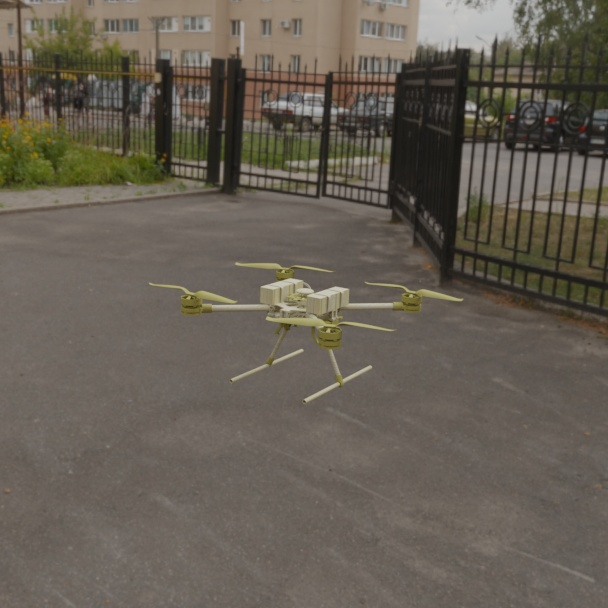
\includegraphics[width=\linewidth,height=2.6cm,keepaspectratio]{graphs/sample_pure_close.jpg}
    \caption{Close-range}
\end{subfigure}\hfill
\begin{subfigure}[t]{0.235\textwidth}
    \centering
    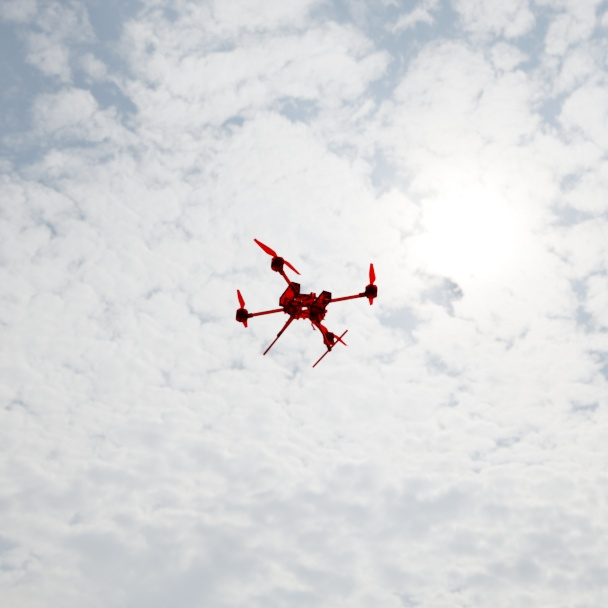
\includegraphics[width=\linewidth,height=2.6cm,keepaspectratio]{graphs/sample_pure_medium.jpg}
    \caption{Mid-range}
\end{subfigure}\hfill
\begin{subfigure}[t]{0.235\textwidth}
    \centering
    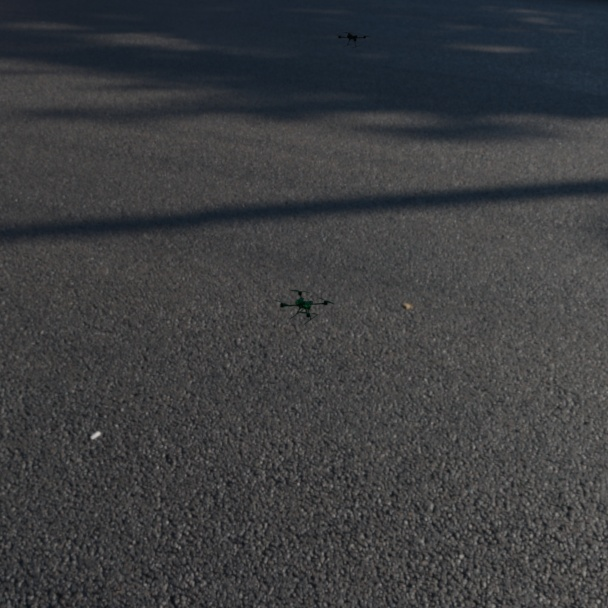
\includegraphics[width=\linewidth,height=2.6cm,keepaspectratio]{graphs/sample_pure_far.jpg}
    \caption{Long-range}
\end{subfigure}\hfill
\begin{subfigure}[t]{0.235\textwidth}
    \centering
    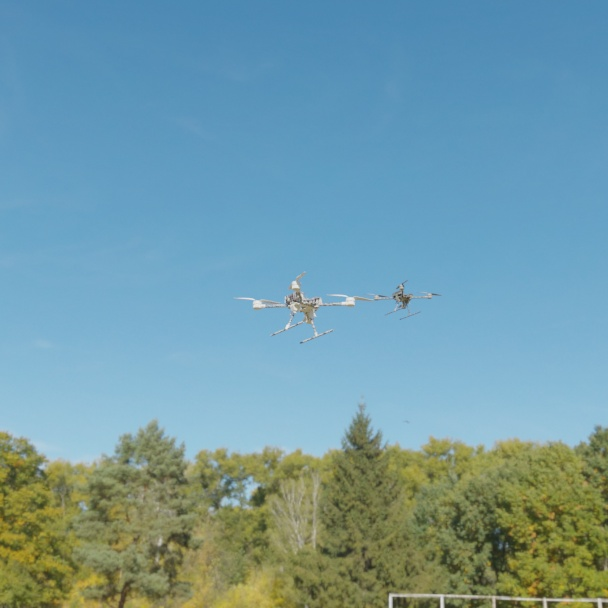
\includegraphics[width=\linewidth,height=2.6cm,keepaspectratio]{graphs/sample_mixed.jpg}
    \caption{Multi-range}
\end{subfigure}
\caption{Sample validation images from each distance category.}
\label{fig:dist-samples}
\end{figure}


\subsection{How many images fall into each category}
The actual counts produced by the script on our validation set are shown in
Table~\ref{tab:dist-counts}. Most of the validation images fall into the
\emph{long-range} category, which is consistent with the fact that drones in
real recordings are often filmed from far away.

\begin{table}[H]
\centering
\caption{Distance-wise category distribution of the validation set.}
\label{tab:dist-counts}
\begin{tabular}{lcc}
\toprule
\textbf{Category}                & \textbf{\#Images} & \textbf{\# Boxes} \\
\midrule
Close-range  (pure close)        &  460  &  506  \\
Mid-range    (pure medium)       &  521  &  699  \\
Long-range   (pure far)          & 1471  & 2354  \\
Multi-range  (mixed)             &   86  &  --   \\
\midrule
\textbf{Total}                   & \textbf{2538} & \textbf{3559} \\
\bottomrule
\end{tabular}
\end{table}

\section{Environment-Wise Validation Split}
\label{sec:env-split}
A second split of the validation set was made on the basis of the
\emph{environment} in which the image was taken. The motivation is the same as
for the distance split: a single average score does not tell us whether the
model is good at clear sky scenes, low-light scenes, or cluttered backgrounds.
Every validation image was therefore assigned to exactly one of three
environment categories described below.

\subsection{Categories}
\begin{itemize}[noitemsep]
    \item \textbf{Clear-sky (bright clear):} Bright, clearly visible images with a simple background, mostly open sky. The drone stands out against a clean backdrop, which usually makes detection easier.
    \item \textbf{Cluttered:} images with a busy, complex background such as
          buildings, trees or roads. Many distractors are present, so the
          detector has to be careful not to produce false positives.
    \item \textbf{Night / low-light:} images captured in
          dim conditions, at dusk or at night. Contrast is low and noise is
          high.
\end{itemize}

\begin{figure}[H]
\centering
\begin{subfigure}[t]{0.31\textwidth}
    \centering
    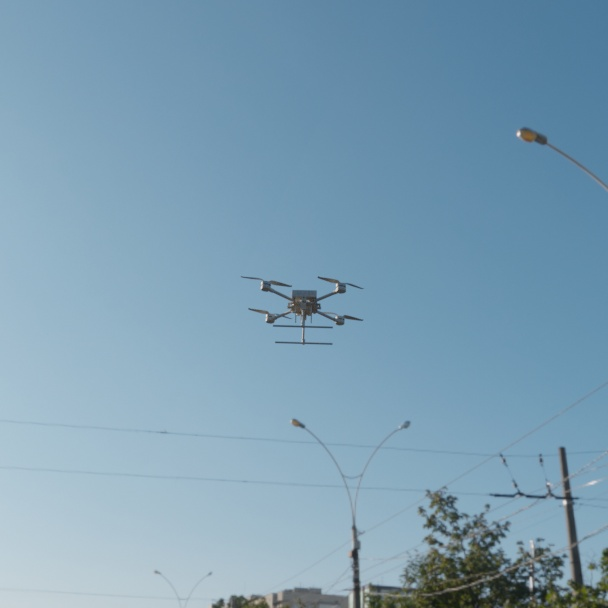
\includegraphics[width=\linewidth,height=3.2cm,keepaspectratio]{graphs/sample_bright_clear.jpg}
    \caption{Clear-sky}
\end{subfigure}\hfill
\begin{subfigure}[t]{0.31\textwidth}
    \centering
    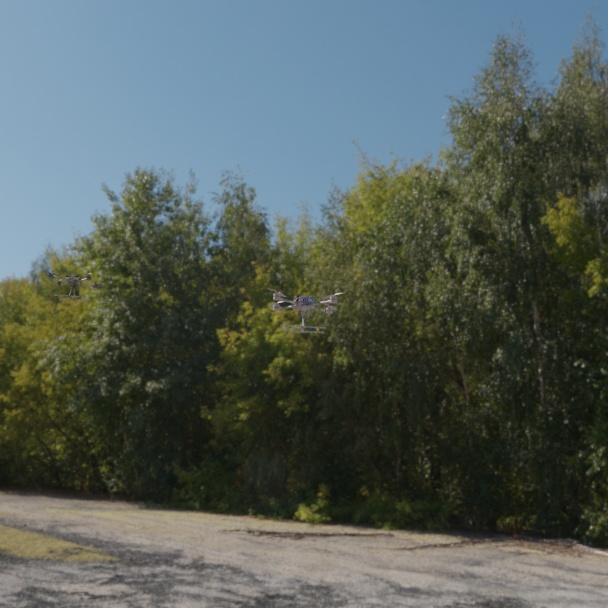
\includegraphics[width=\linewidth,height=3.2cm,keepaspectratio]{graphs/sample_cluttered.jpg}
    \caption{Cluttered}
\end{subfigure}\hfill
\begin{subfigure}[t]{0.31\textwidth}
    \centering
    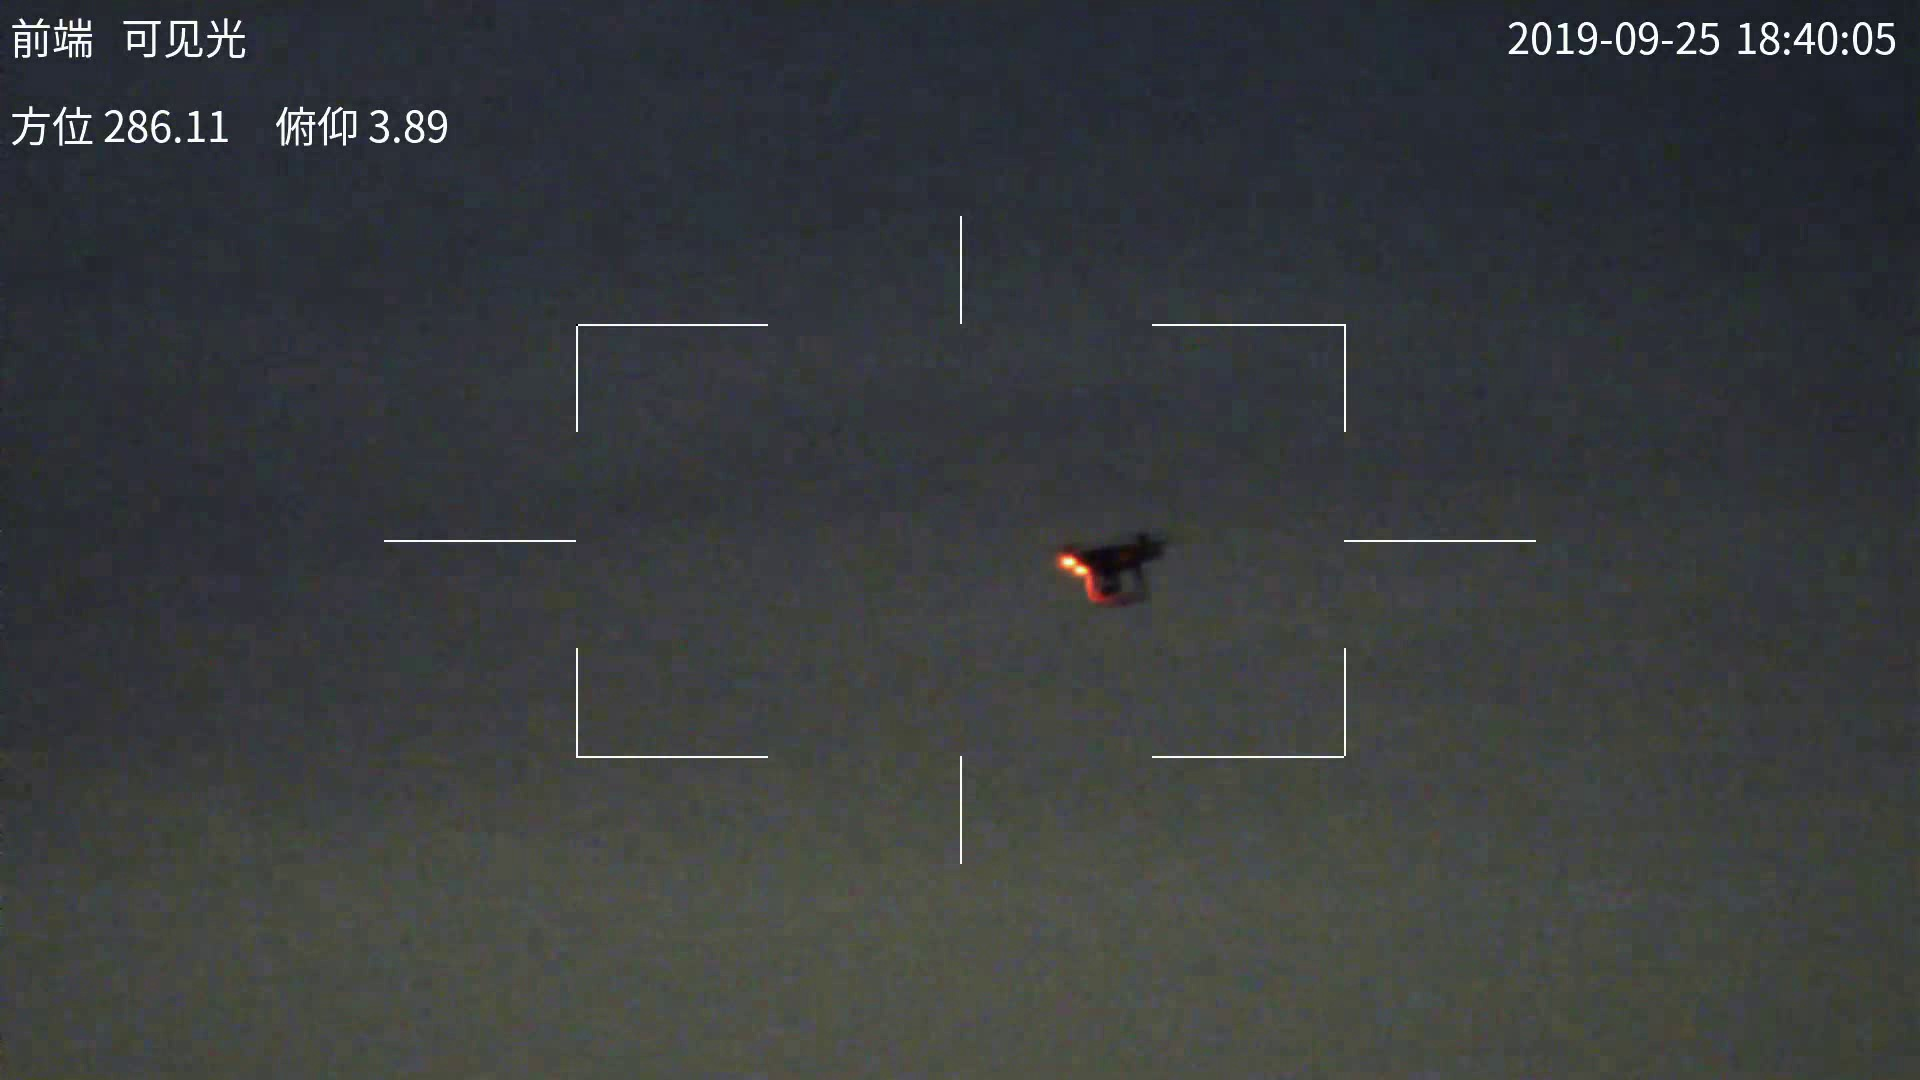
\includegraphics[width=\linewidth,height=3.2cm,keepaspectratio]{graphs/sample_lowlight.jpg}
    \caption{Low-light}
\end{subfigure}
\caption{Sample validation images from each environment category.}
\label{fig:env-samples}
\end{figure}

\subsection{How many images fall into each category}
Table~\ref{tab:env-counts} shows the actual numbers. Almost half of the
validation images turn out to be \emph{cluttered}, which is the hardest
setting for any detector and therefore an important case to evaluate
separately.

\begin{table}[H]
\centering
\caption{Environment-wise category distribution of the validation set.}
\label{tab:env-counts}
\begin{tabular}{lcc}
\toprule
\textbf{Category}                  & \textbf{\# Images} & \textbf{\% of val set} \\
\midrule
Clear-sky    (bright clear)        &  682 & 26.86\,\% \\
Low-light    (night / low-light)   &  584 & 23.00\,\% \\
Cluttered                          & 1273 & 50.14\,\% \\
\midrule
\textbf{Total}                     & \textbf{2539} & \textbf{100.00\,\%} \\
\bottomrule
\end{tabular}
\end{table}



% =====================================================================
%  CHAPTER 4 — METHODOLOGY AND RESULTS
% =====================================================================
\chapter{Methodology and Experimental Results}
\label{ch:expts}

This chapter describes how the model was trained and presents the results in
one place: training curves first, then the distance-wise and environment-wise
results, and finally the comparison with the earlier existing model.

% --------------------------------------------------
\section{Model and Training Setup}

\subsection{Model: YOLO11-Nano}
The model used in all experiments is \textbf{YOLO11-nano} (\texttt{yolo11n}),
the smallest variant of the YOLO11 family. The reasons for choosing it were
explained in Chapter~\ref{ch:related}. Briefly, it provides:
\begin{itemize}[noitemsep]
    \item An anchor-free detection head with a dual-task prediction design.
    \item The C3k2 block in the backbone for fast feature extraction.
    \item The C2PSA attention block, which helps with small targets.
    \item Three loss terms during training: a box regression loss, a
          classification loss, and a Distribution Focal Loss (DFL).
\end{itemize}

\subsection{YOLO11 Pipeline at a Glance}
At a high level, YOLO11 takes a single RGB image and produces a list of
bounding boxes with class labels in one forward pass. The diagram below shows
the main stages the image goes through inside the network:

\begin{figure}[H]
\centering
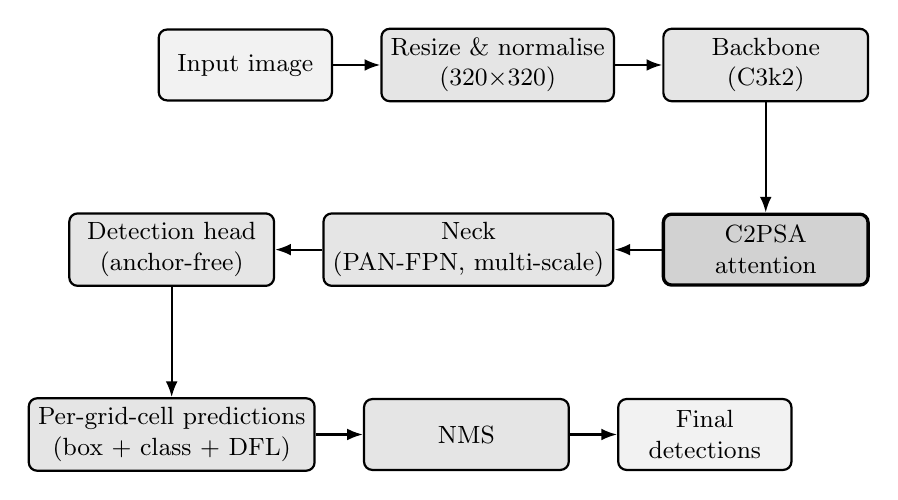
\begin{tikzpicture}[
    font=\small,
    node distance=8mm and 6mm,
    every node/.style={align=center},
    io/.style   ={rectangle, rounded corners=3pt, draw, thick,
                  minimum width=22mm, minimum height=9mm, fill=gray!10},
    proc/.style ={rectangle, rounded corners=3pt, draw, thick,
                  minimum width=26mm, minimum height=9mm, fill=gray!20},
    attn/.style ={rectangle, rounded corners=3pt, draw, very thick,
                  minimum width=26mm, minimum height=9mm, fill=gray!35},
    arr/.style  ={-{Latex[length=2mm]}, thick}
]
% Row 1
\node[io]   (img)     {Input image};
\node[proc, right=of img]  (pre)     {Resize \& normalise\\(320$\times$320)};
\node[proc, right=of pre]  (back)    {Backbone\\(C3k2)};

% Row 2
\node[attn, below=14mm of back]  (attn)    {C2PSA\\attention};
\node[proc, left=of attn]        (neck)    {Neck\\(PAN-FPN, multi-scale)};
\node[proc, left=of neck]        (head)    {Detection head\\(anchor-free)};

% Row 3
\node[proc, below=14mm of head]  (pred)    {Per-grid-cell predictions\\(box + class + DFL)};
\node[proc, right=of pred]       (nms)     {NMS};
\node[io,   right=of nms]        (out)     {Final\\detections};

% Arrows row 1
\draw[arr] (img)  -- (pre);
\draw[arr] (pre)  -- (back);
% down to row 2
\draw[arr] (back.south) -- ++(0,-3mm) -| (attn.north);
% row 2 (right to left)
\draw[arr] (attn) -- (neck);
\draw[arr] (neck) -- (head);
% down to row 3
\draw[arr] (head.south) -- ++(0,-3mm) -| (pred.north);
% row 3
\draw[arr] (pred) -- (nms);
\draw[arr] (nms)  -- (out);
\end{tikzpicture}
\caption{High-level pipeline of YOLO11.}
\label{fig:yolo-pipeline}
\end{figure}

A short description of each stage:
\begin{itemize}[noitemsep]
    \item \textbf{Input image \& preprocessing.} The RGB image is resized to a
          fixed size ($320\times320$ in our setup) and pixel values are
          normalised to the range $[0, 1]$.
    \item \textbf{Backbone (C3k2).} A stack of convolutional blocks extracts
          features at multiple scales. The C3k2 block is a lighter, faster
          variant of the older C3 block.
    \item \textbf{C2PSA attention.} A spatial attention block that lets the
          network put more weight on small, scattered regions -- exactly the
          parts of the image where distant drones tend to appear.
    \item \textbf{Neck (PAN-FPN).} A Path Aggregation Network combines features
          from different depths so that small objects (from shallow, high-resolution
          maps) and large objects (from deep, low-resolution maps) are both
          handled well.
    \item \textbf{Detection head (anchor-free).} The image is implicitly
          divided into a grid. For each grid cell at each scale, the head
          directly predicts a bounding box, an object/class score, and a DFL
          distribution that helps refine the box edges.
    \item \textbf{NMS.} Non-Maximum Suppression removes overlapping duplicate
          boxes for the same drone, leaving one final detection per object.
\end{itemize}

\subsection{Training Hyperparameters}
The hyperparameters were chosen to fit the available memory while keeping
the training stable.

\begin{table}[H]
\centering
\caption{Training hyperparameters used for both phases.}
\label{tab:hyperparams}
\begin{tabular}{ll}
\toprule
\textbf{Parameter}      & \textbf{Value} \\
\midrule
Model weights           & \texttt{yolo11n} \\
Image size              & $320 \times 320$ \\
Batch size              & 2 \\
Workers                 & 1 \\
Confidence threshold    & 0.25 \\
Early-stopping patience & 30 epochs \\
Optimiser               & AdamW (Ultralytics default) \\
Hardware                & Single shared GPU \\
\bottomrule
\end{tabular}
\end{table}

\subsection{Two-Phase Training Strategy}
The model was first trained for 200 epochs from the pretrained
\texttt{yolo11n} weights. Looking at the training curves around epoch~180, the
loss was still showing a noticeable downward trend, which suggested that the
model had not yet fully converged and that more training would still help. To
take advantage of this, the training was resumed from the Phase~1 checkpoint
and continued for another 300 epochs, giving a total of 500 epochs split into
two phases.

\begin{table}[H]
\centering
\caption{Two-phase training schedule.}
\label{tab:phases}
\begin{tabular}{lcc}
\toprule
\textbf{}                & \textbf{Phase 1}               & \textbf{Phase 2} \\
\midrule
Epoch range              & 1\,--\,200                     & 201\,--\,500 \\
Number of epochs         & 200                            & 300 \\
Starting weights         & \texttt{yolo11n} (fresh)       & Phase~1 \texttt{last.pt} \\
Image size               & 320                            & 320 \\
Batch size               & 2                              & 2 \\
Patience                 & 30                             & 30 \\
\bottomrule
\end{tabular}
\end{table}

Phase~2 resumes training from the last Phase~1 checkpoint so that the optimizer
state and learnt features are preserved, and the network is then fine-tuned for
another 300 epochs.

\subsection{Evaluation Metrics}
The standard object-detection metrics are used to evaluate the trained model.

\begin{itemize}[noitemsep]
    \item \textbf{Precision}, $P = \tfrac{TP}{TP+FP}$: out of all the boxes the
          model predicted as drones, the fraction that were actually drones.
          High precision means few false alarms.
    \item \textbf{Recall}, $R = \tfrac{TP}{TP+FN}$: out of all the real drones
          in the images, the fraction the model managed to find. High recall
          means few missed drones.
    \item \textbf{mAP@50}: mean Average Precision at an IoU threshold of
          $0.50$ -- a box counts as correct if it overlaps the ground truth by
          at least $50\%$. It mainly checks whether the drone was found.
    \item \textbf{mAP@50\,--\,95}: mean AP averaged over IoU thresholds from
          $0.50$ to $0.95$ in steps of $0.05$. The stricter thresholds also
          reward the model for drawing tight, well-localised boxes.
\end{itemize}

% --------------------------------------------------
\section{Training Curves}

Figure~\ref{fig:training-losses-combined} shows the three loss components
across the full 500-epoch schedule. The vertical dashed line marks the
transition from Phase~1 to Phase~2. There is a small expected jump at epoch~201
when training is resumed, after which all three losses decrease again.

\begin{figure}[H]
\centering
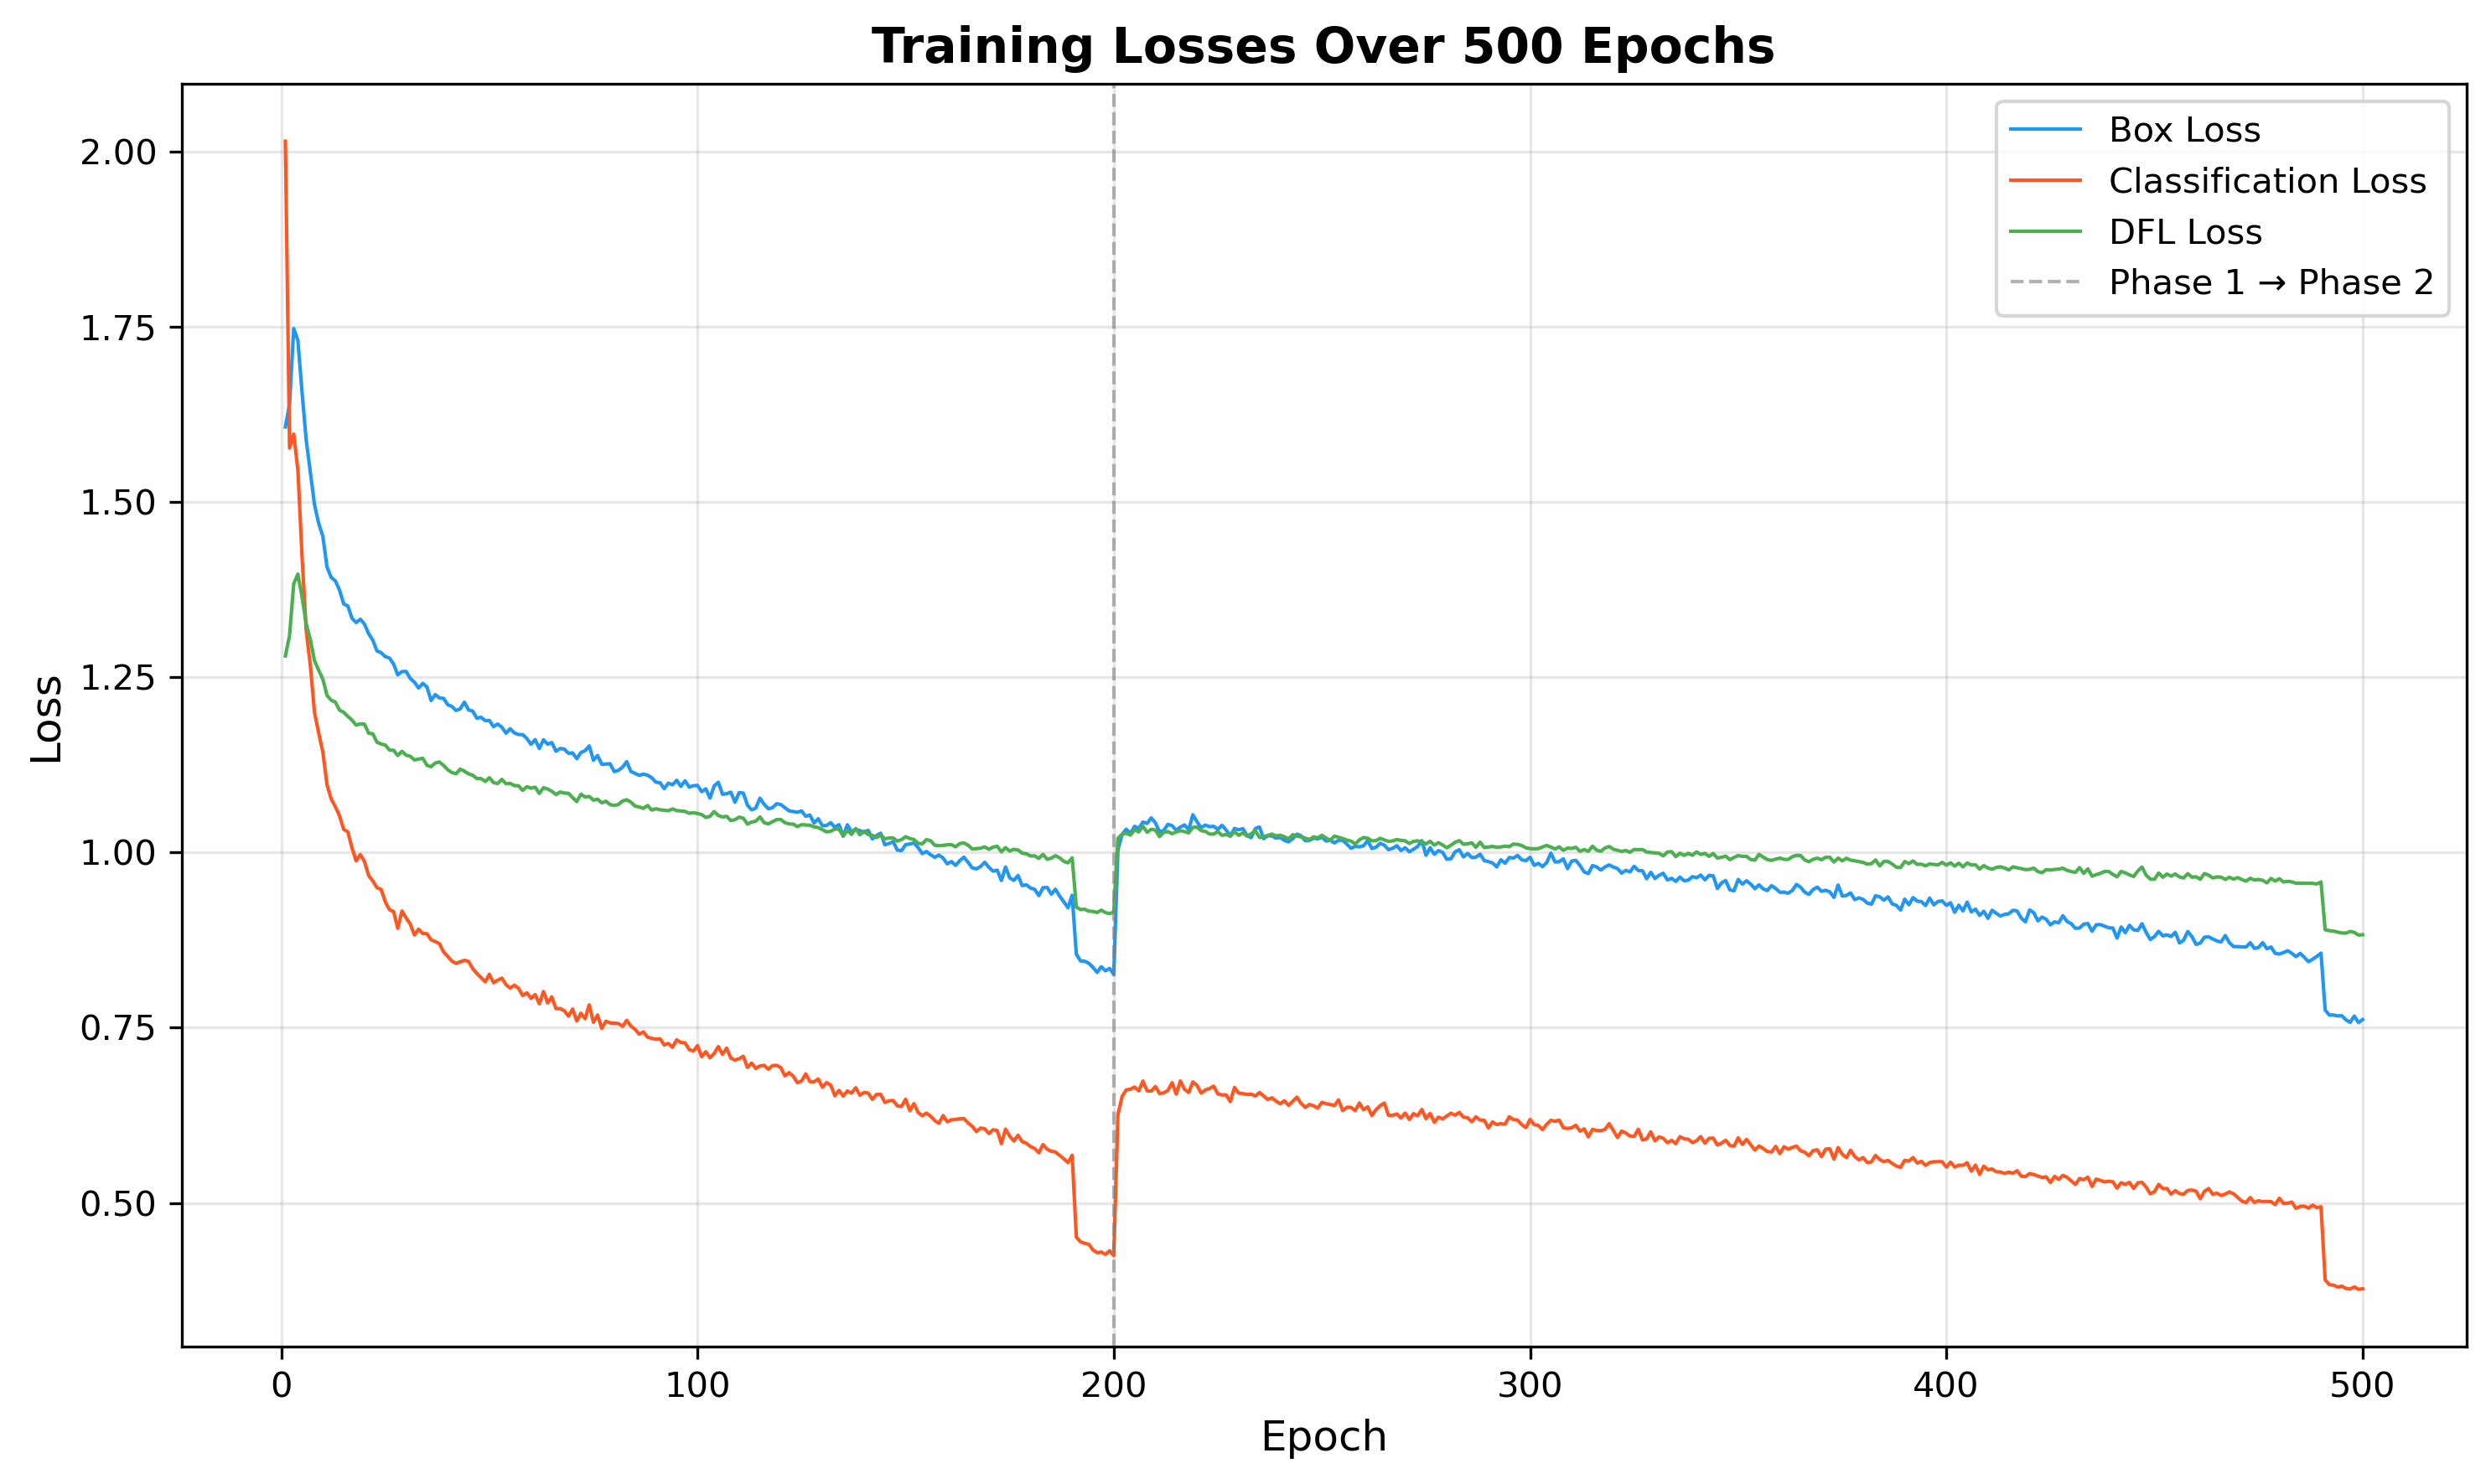
\includegraphics[width=0.95\textwidth]{graphs/training_losses_combined.png}
\caption{Training loss components (Box, Classification, DFL) over 500 epochs.}
\label{fig:training-losses-combined}
\end{figure}

\begin{table}[H]
\centering
\caption{Training loss values at key milestones.}
\label{tab:loss-milestones}
\begin{tabular}{lccc}
\toprule
\textbf{Epoch}     & \textbf{Box loss} & \textbf{Cls loss} & \textbf{DFL loss} \\
\midrule
1                  & 1.6071 & 2.0148 & 1.2804 \\
50                 & 1.1883 & 0.8263 & 1.1066 \\
100                & 1.0957 & 0.7244 & 1.0556 \\
150                & 1.0111 & 0.6479 & 1.0224 \\
200 (Phase~1 end)  & 0.8346 & 0.4317 & 0.9126 \\
250                & 1.0216 & 0.6435 & 1.0245 \\
300                & 0.9930 & 0.6191 & 1.0054 \\
400                & 0.9245 & 0.5511 & 0.9819 \\
500 (Phase~2 end)  & 0.7614 & 0.3774 & 0.8826 \\
\bottomrule
\end{tabular}
\end{table}

Figure~\ref{fig:map-curves} and Figure~\ref{fig:pr-curves} show the
mAP and the precision/recall curves over the same 500 epochs. Both curves
follow the same overall pattern: a fast rise during the first $\sim$50 epochs,
slow improvement from then up to epoch~200, the small Phase~2 reset, and a
gradual climb again.

\begin{figure}[H]
\centering
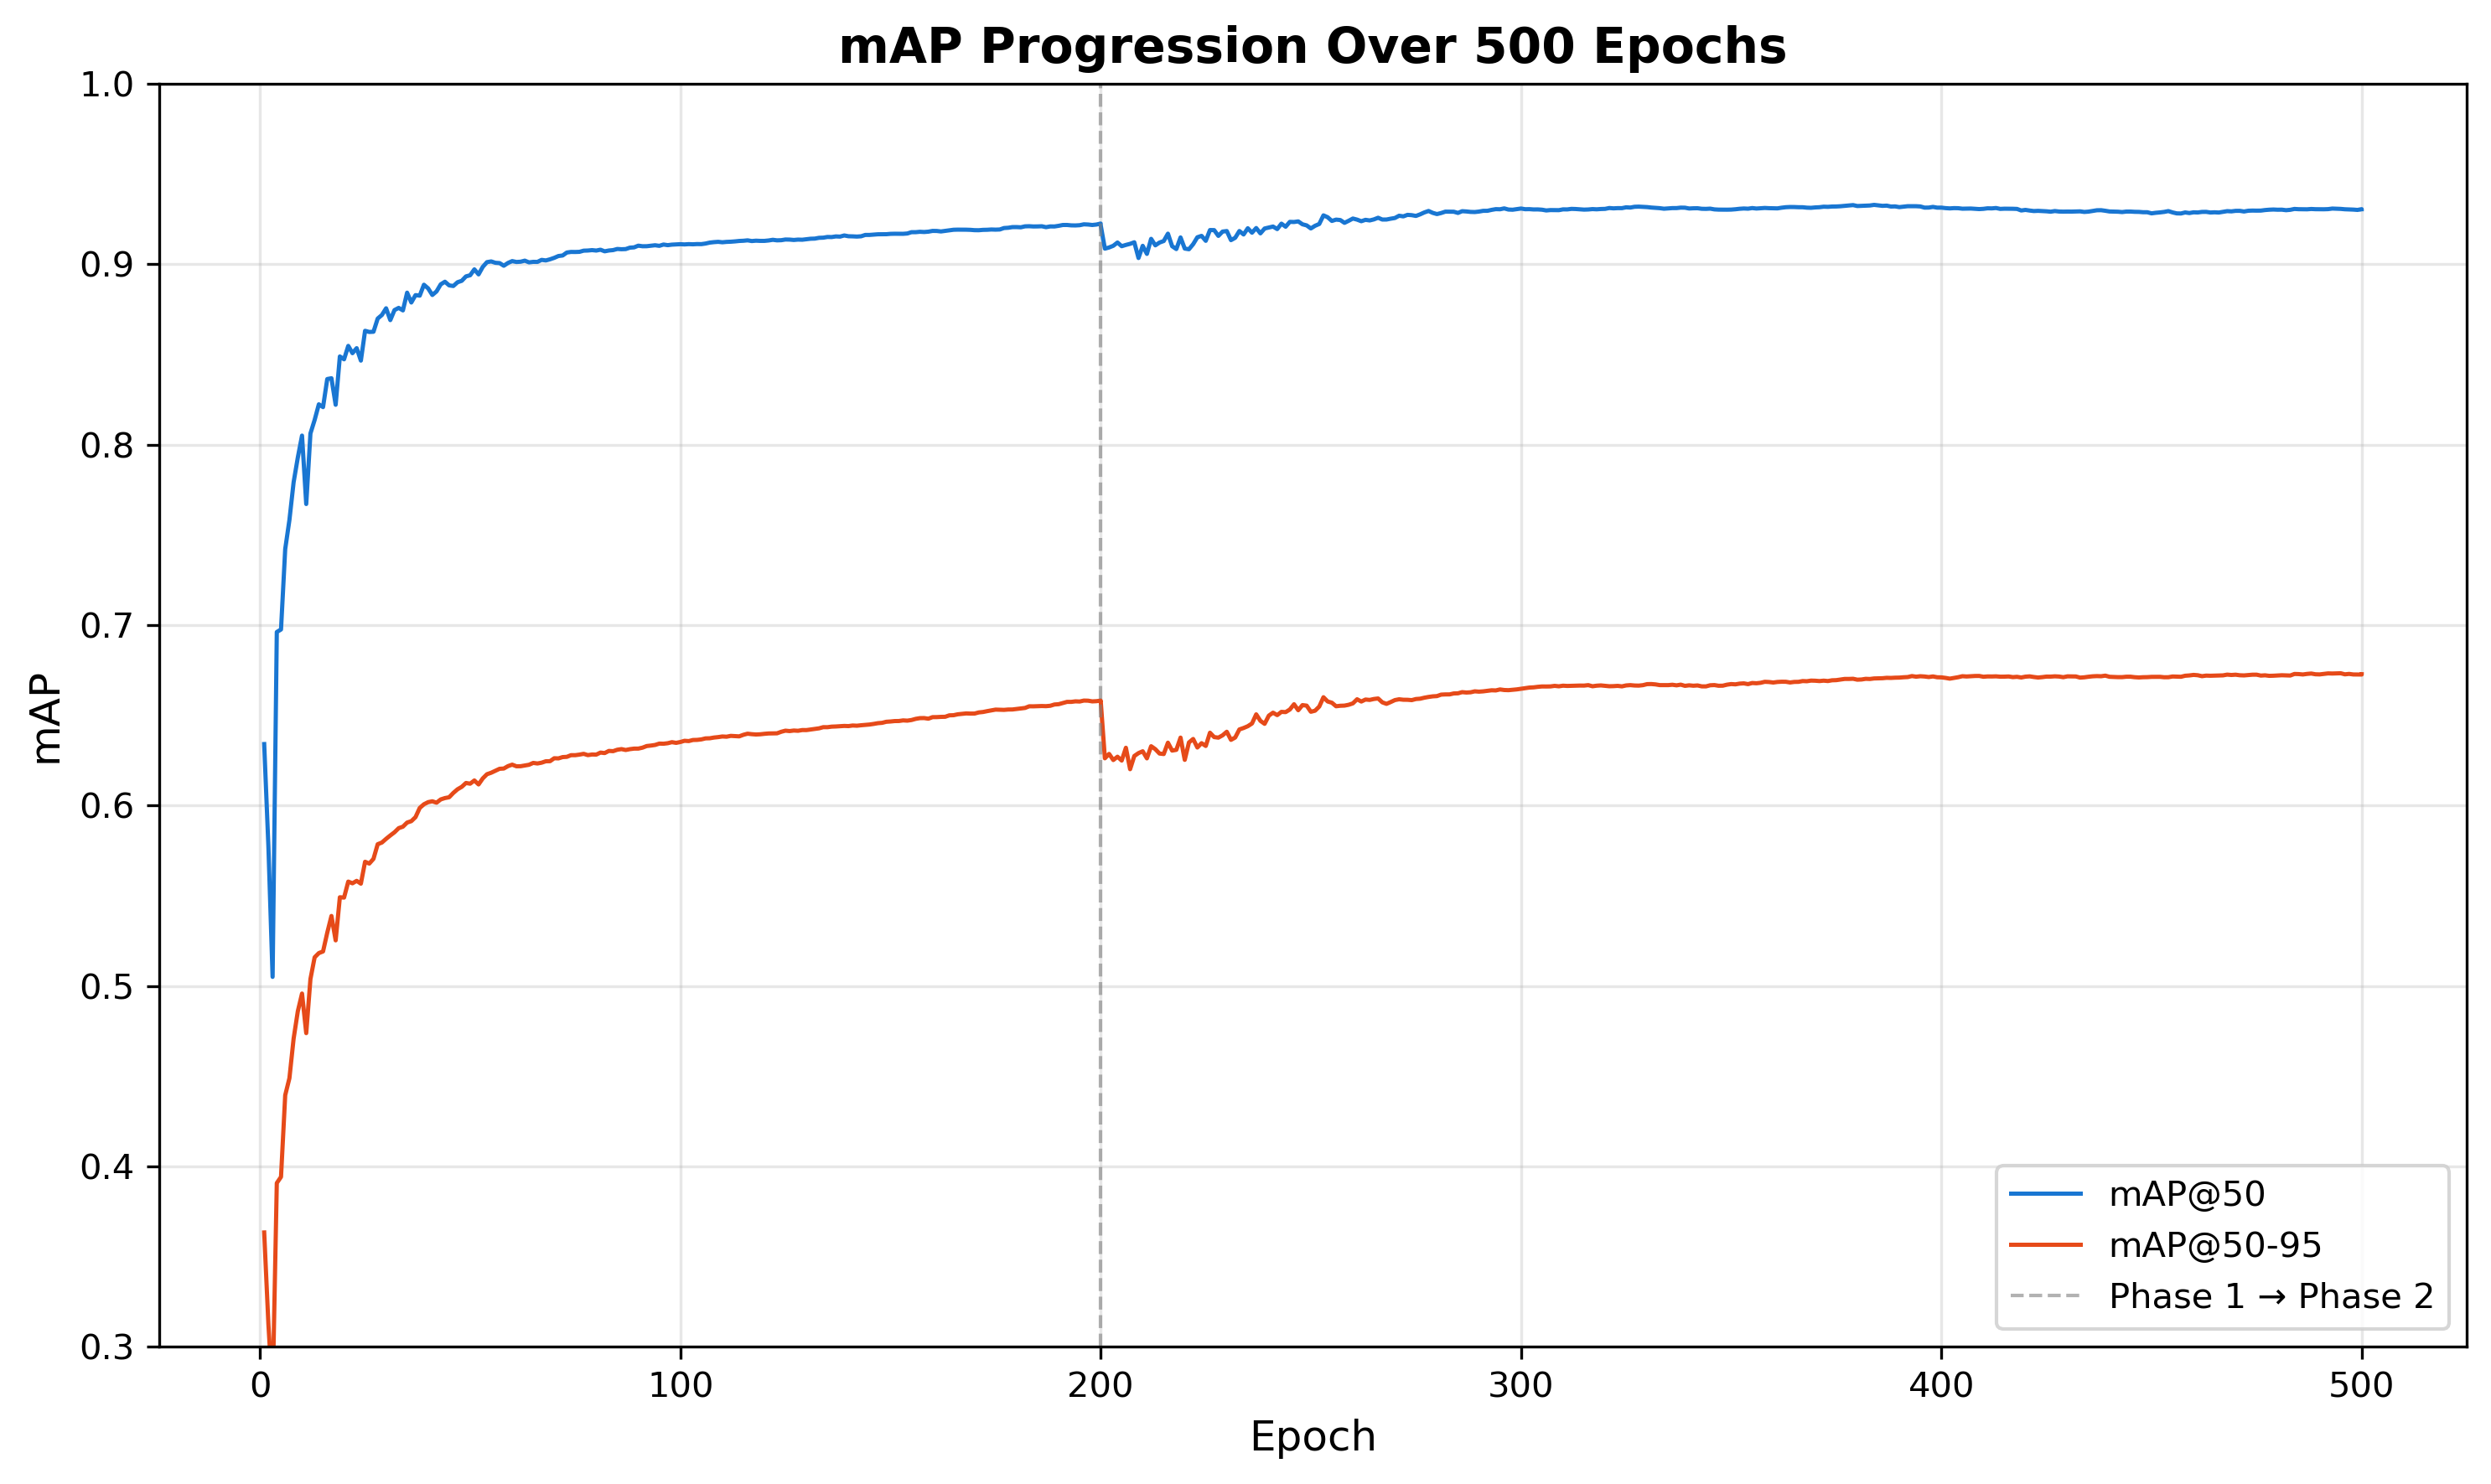
\includegraphics[width=0.9\textwidth]{graphs/map_curves.png}
\caption{mAP@50 and mAP@50\,--\,95 progression over 500 epochs.}
\label{fig:map-curves}
\end{figure}

\begin{figure}[H]
\centering
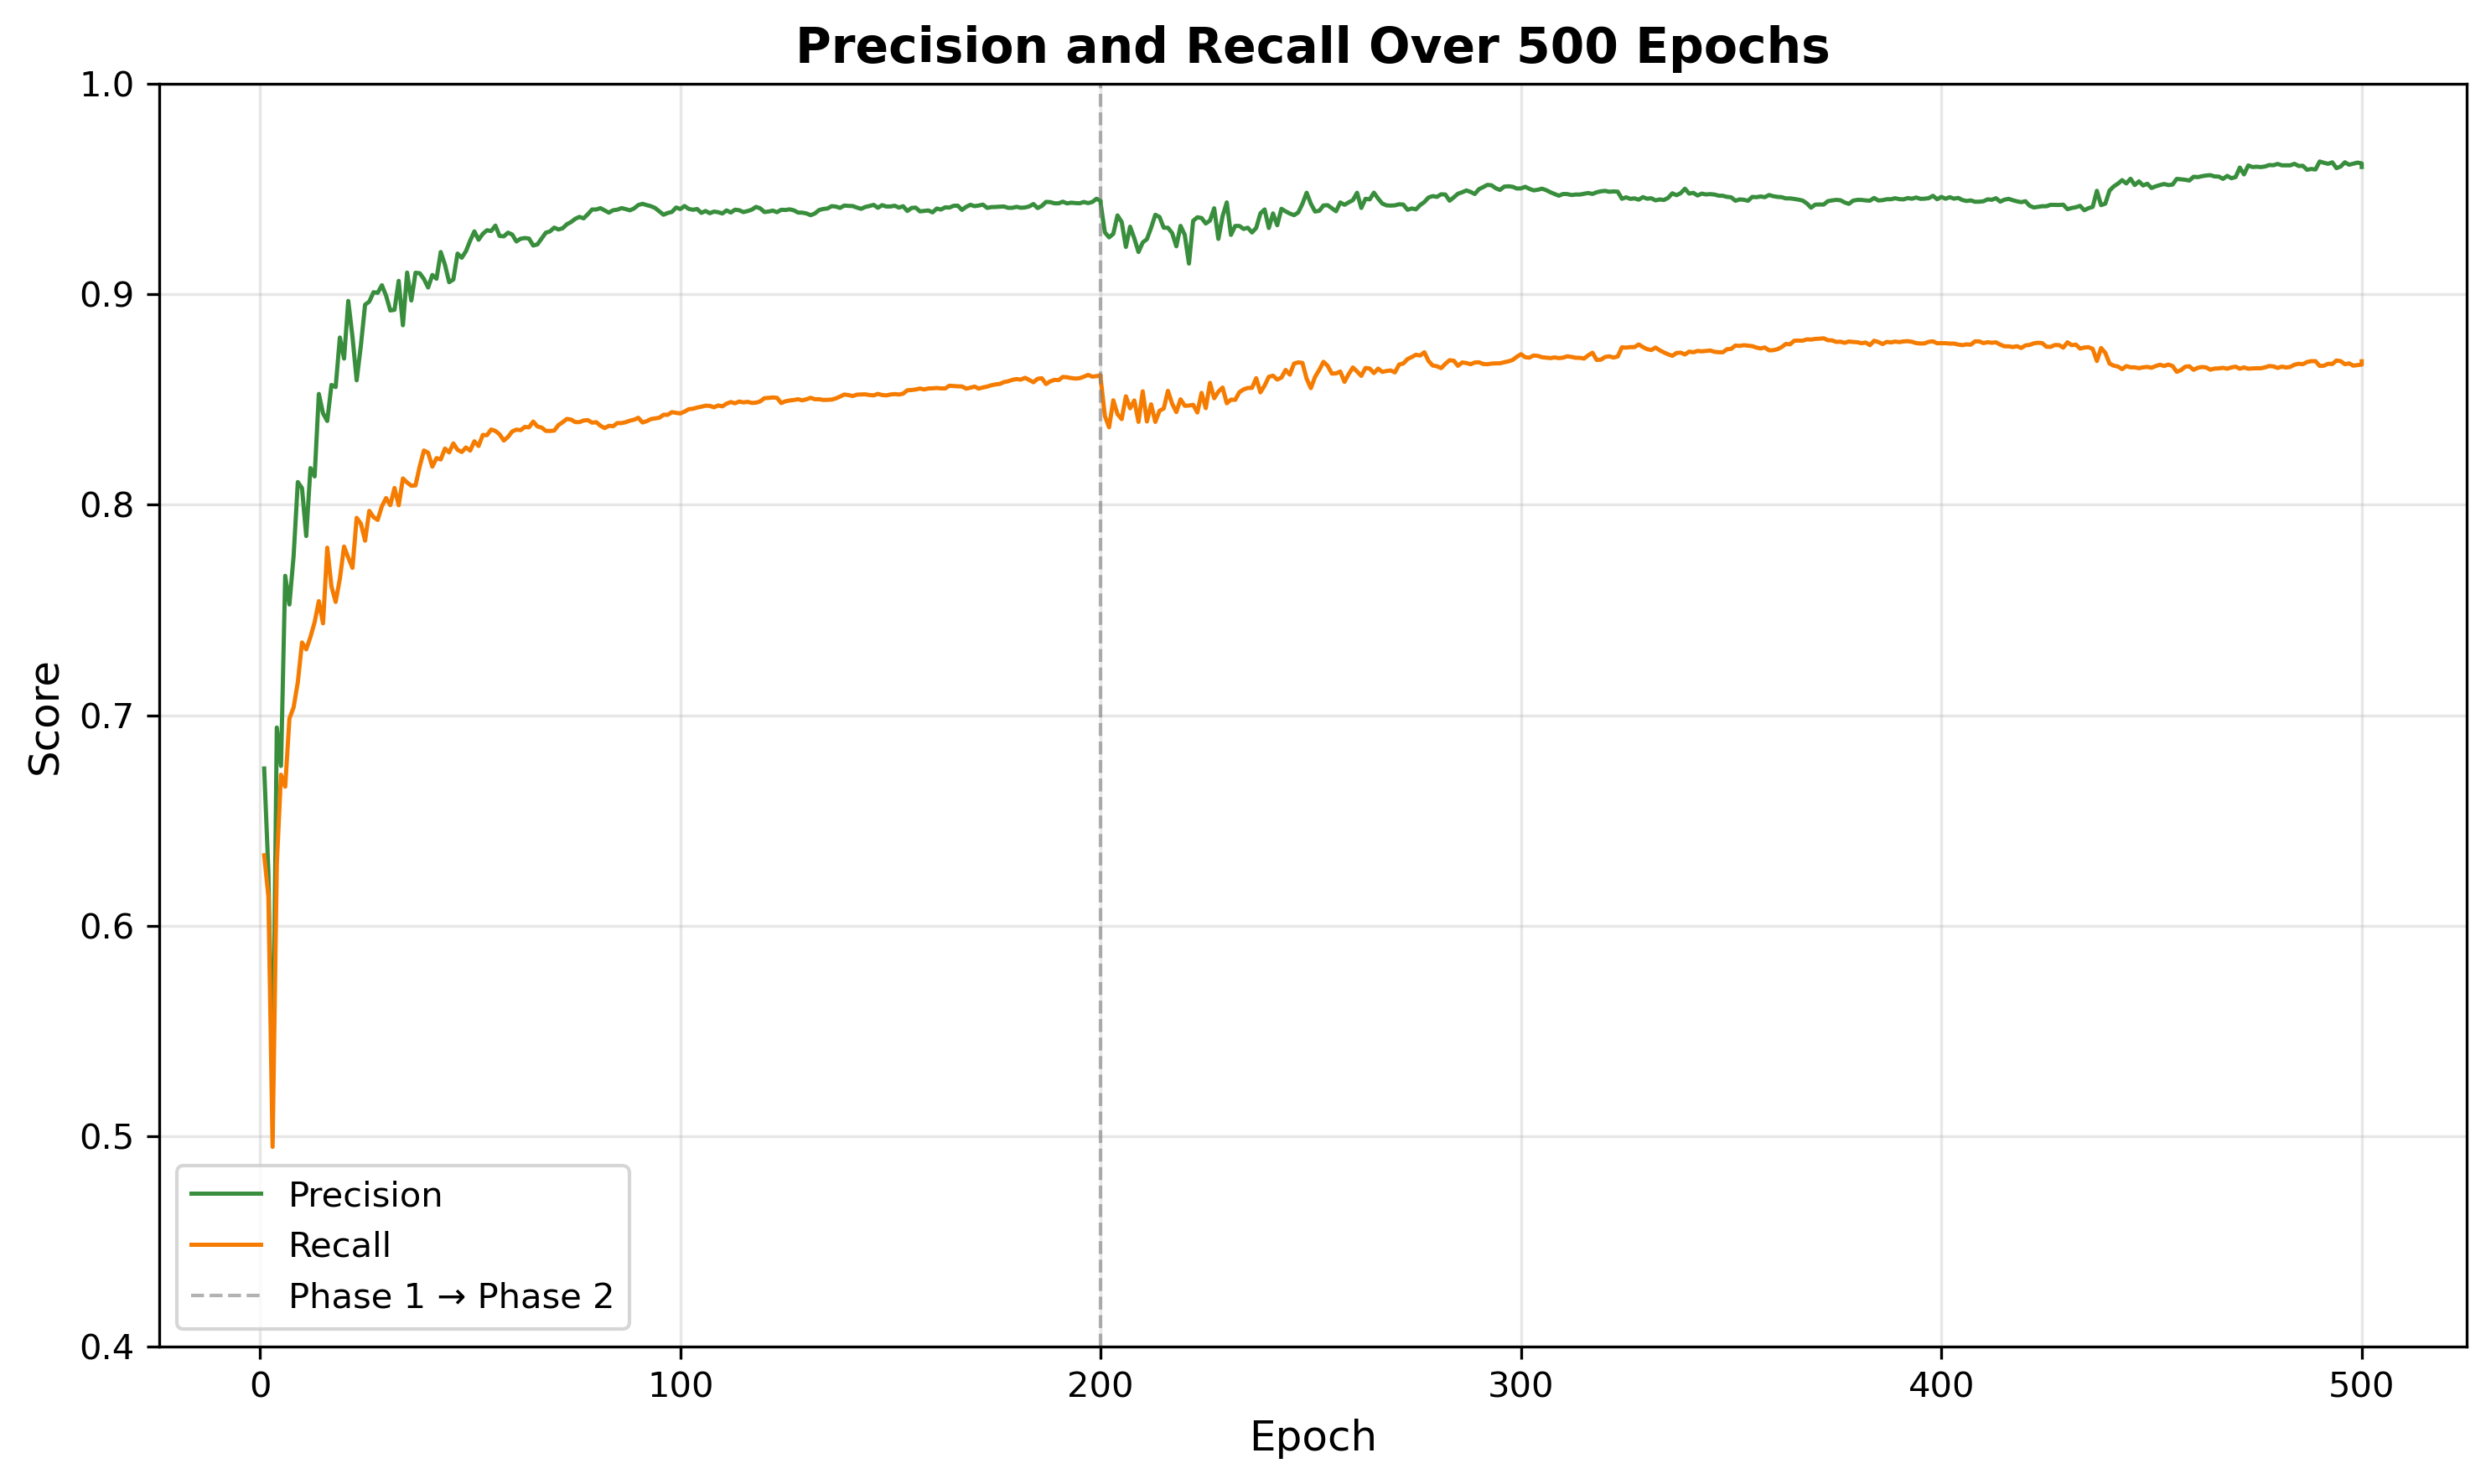
\includegraphics[width=0.9\textwidth]{graphs/precision_recall_curves.png}
\caption{Precision and Recall progression over 500 epochs.}
\label{fig:pr-curves}
\end{figure}

\begin{table}[H]
\centering
\caption{Validation metrics at key milestones.}
\label{tab:val-milestones}
\begin{tabular}{lcccc}
\toprule
\textbf{Epoch}     & \textbf{Precision} & \textbf{Recall} & \textbf{mAP@50} & \textbf{mAP@50\,--\,95} \\
\midrule
1                  & 0.6747 & 0.6335 & 0.6340 & 0.3633 \\
50                 & 0.9255 & 0.8257 & 0.8939 & 0.6121 \\
100                & 0.9405 & 0.8434 & 0.9111 & 0.6352 \\
150                & 0.9417 & 0.8524 & 0.9168 & 0.6465 \\
200 (Phase~1 end)  & 0.9454 & 0.8611 & 0.9220 & 0.6578 \\
300                & 0.9503 & 0.8716 & 0.9309 & 0.6647 \\
400                & 0.9463 & 0.8768 & 0.9314 & 0.6710 \\
500 (Phase~2 end)  & 0.9622 & 0.8662 & 0.9305 & 0.6727 \\
\bottomrule
\end{tabular}
\end{table}

\subsection{Phase~1 vs Phase~2}
Figure~\ref{fig:phase-comparison} and Table~\ref{tab:phase-comparison} compare
the final metrics of the two phases.

\begin{figure}[H]
\centering
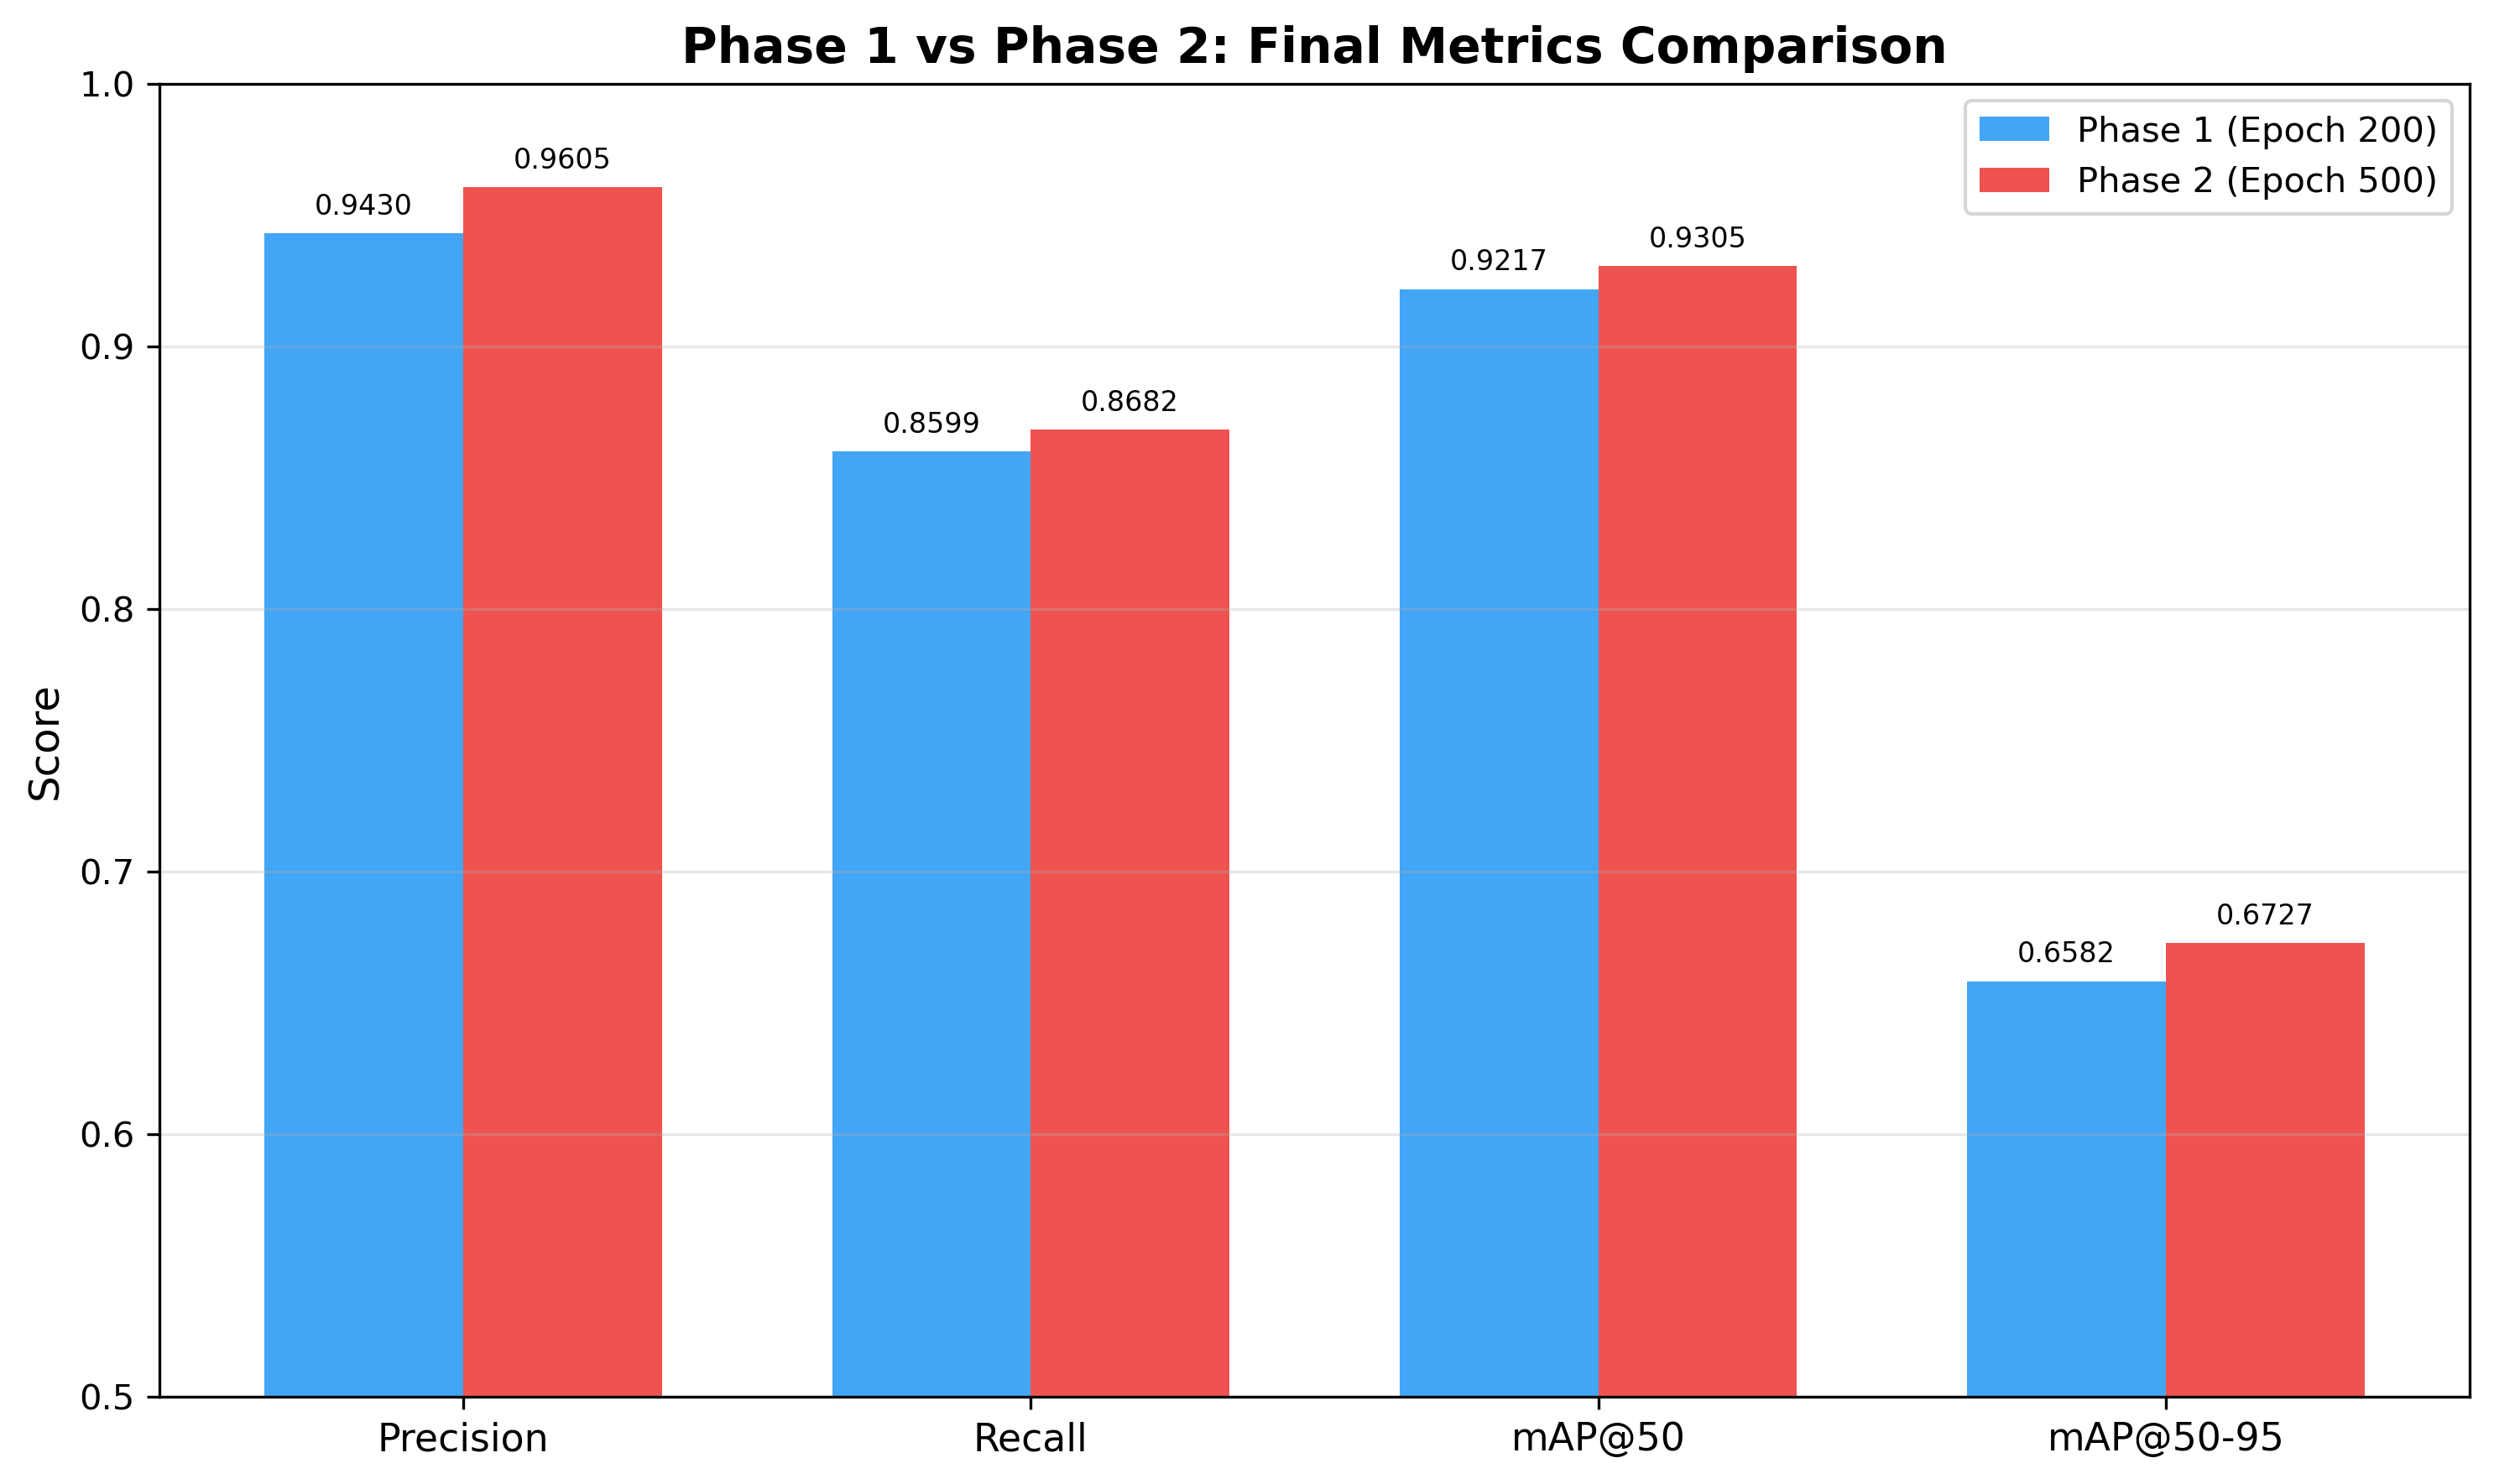
\includegraphics[width=0.85\textwidth]{graphs/phase_comparison.png}
\caption{Phase~1 vs Phase~2 final-metric comparison.}
\label{fig:phase-comparison}
\end{figure}

\begin{table}[H]
\centering
\caption{Final metrics: Phase~1 (epoch 200) vs Phase~2 (epoch 500).}
\label{tab:phase-comparison}
\begin{tabular}{lccc}
\toprule
\textbf{Metric}              & \textbf{Phase~1} & \textbf{Phase~2} & \textbf{Change} \\
\midrule
Precision                    & 0.9454 & 0.9622 & $+1.78\%$ \\
Recall                       & 0.8611 & 0.8662 & $+0.59\%$ \\
mAP@50                       & 0.9220 & 0.9305 & $+0.92\%$ \\
mAP@50\,--\,95               & 0.6578 & 0.6727 & $+2.27\%$ \\
\bottomrule
\end{tabular}
\end{table}

The extra 300 epochs of Phase~2 give a clear improvement in precision
($+1.78\%$) and in mAP@50\,--\,95 ($+2.27\%$). The improvements in mAP@50 and
recall are smaller, which suggests that the model already finds most drones
after Phase~1 and Phase~2 mainly helps it draw tighter and more confident boxes.

% --------------------------------------------------
\section{Distance-Wise Results}
\label{sec:dist-results}

The same model was then validated on each of the four distance subsets defined
in Section~\ref{sec:dist-split}. The results at the end of Phase~1 and Phase~2
are shown in Tables~\ref{tab:dist-phase1} and \ref{tab:dist-phase2}.

\begin{table}[H]
\centering
\caption{Distance-wise validation -- Phase~1 (epoch 200).}
\label{tab:dist-phase1}
\begin{tabular}{lcccc}
\toprule
\textbf{Subset}           & \textbf{P} & \textbf{R} & \textbf{mAP@50} & \textbf{mAP@50\,--\,95} \\
\midrule
Close-range  (pure close) & 0.9669 & 0.9623 & 0.9831 & 0.8548 \\
Mid-range    (pure medium)& 0.9745 & 0.9547 & 0.9795 & 0.7731 \\
Long-range   (pure far)   & 0.9218 & 0.8155 & 0.8784 & 0.5229 \\
Multi-range  (mixed)      & 0.9601 & 0.8696 & 0.9152 & 0.7091 \\
\bottomrule
\end{tabular}
\end{table}

\begin{table}[H]
\centering
\caption{Distance-wise validation -- Phase~2 (epoch 500).}
\label{tab:dist-phase2}
\begin{tabular}{lcccc}
\toprule
\textbf{Subset}           & \textbf{P} & \textbf{R} & \textbf{mAP@50} & \textbf{mAP@50\,--\,95} \\
\midrule
Close-range  (pure close) & 0.9533 & 0.8852 & 0.9534 & 0.8322 \\
Mid-range    (pure medium)& \textbf{0.9843} & \textbf{0.9690} & \textbf{0.9889} & \textbf{0.8003} \\
Long-range   (pure far)   & 0.9496 & 0.8479 & 0.9066 & 0.5502 \\
Multi-range  (mixed)      & 0.9579 & 0.8810 & 0.9273 & 0.7249 \\
\bottomrule
\end{tabular}
\end{table}

\begin{figure}[H]
\centering
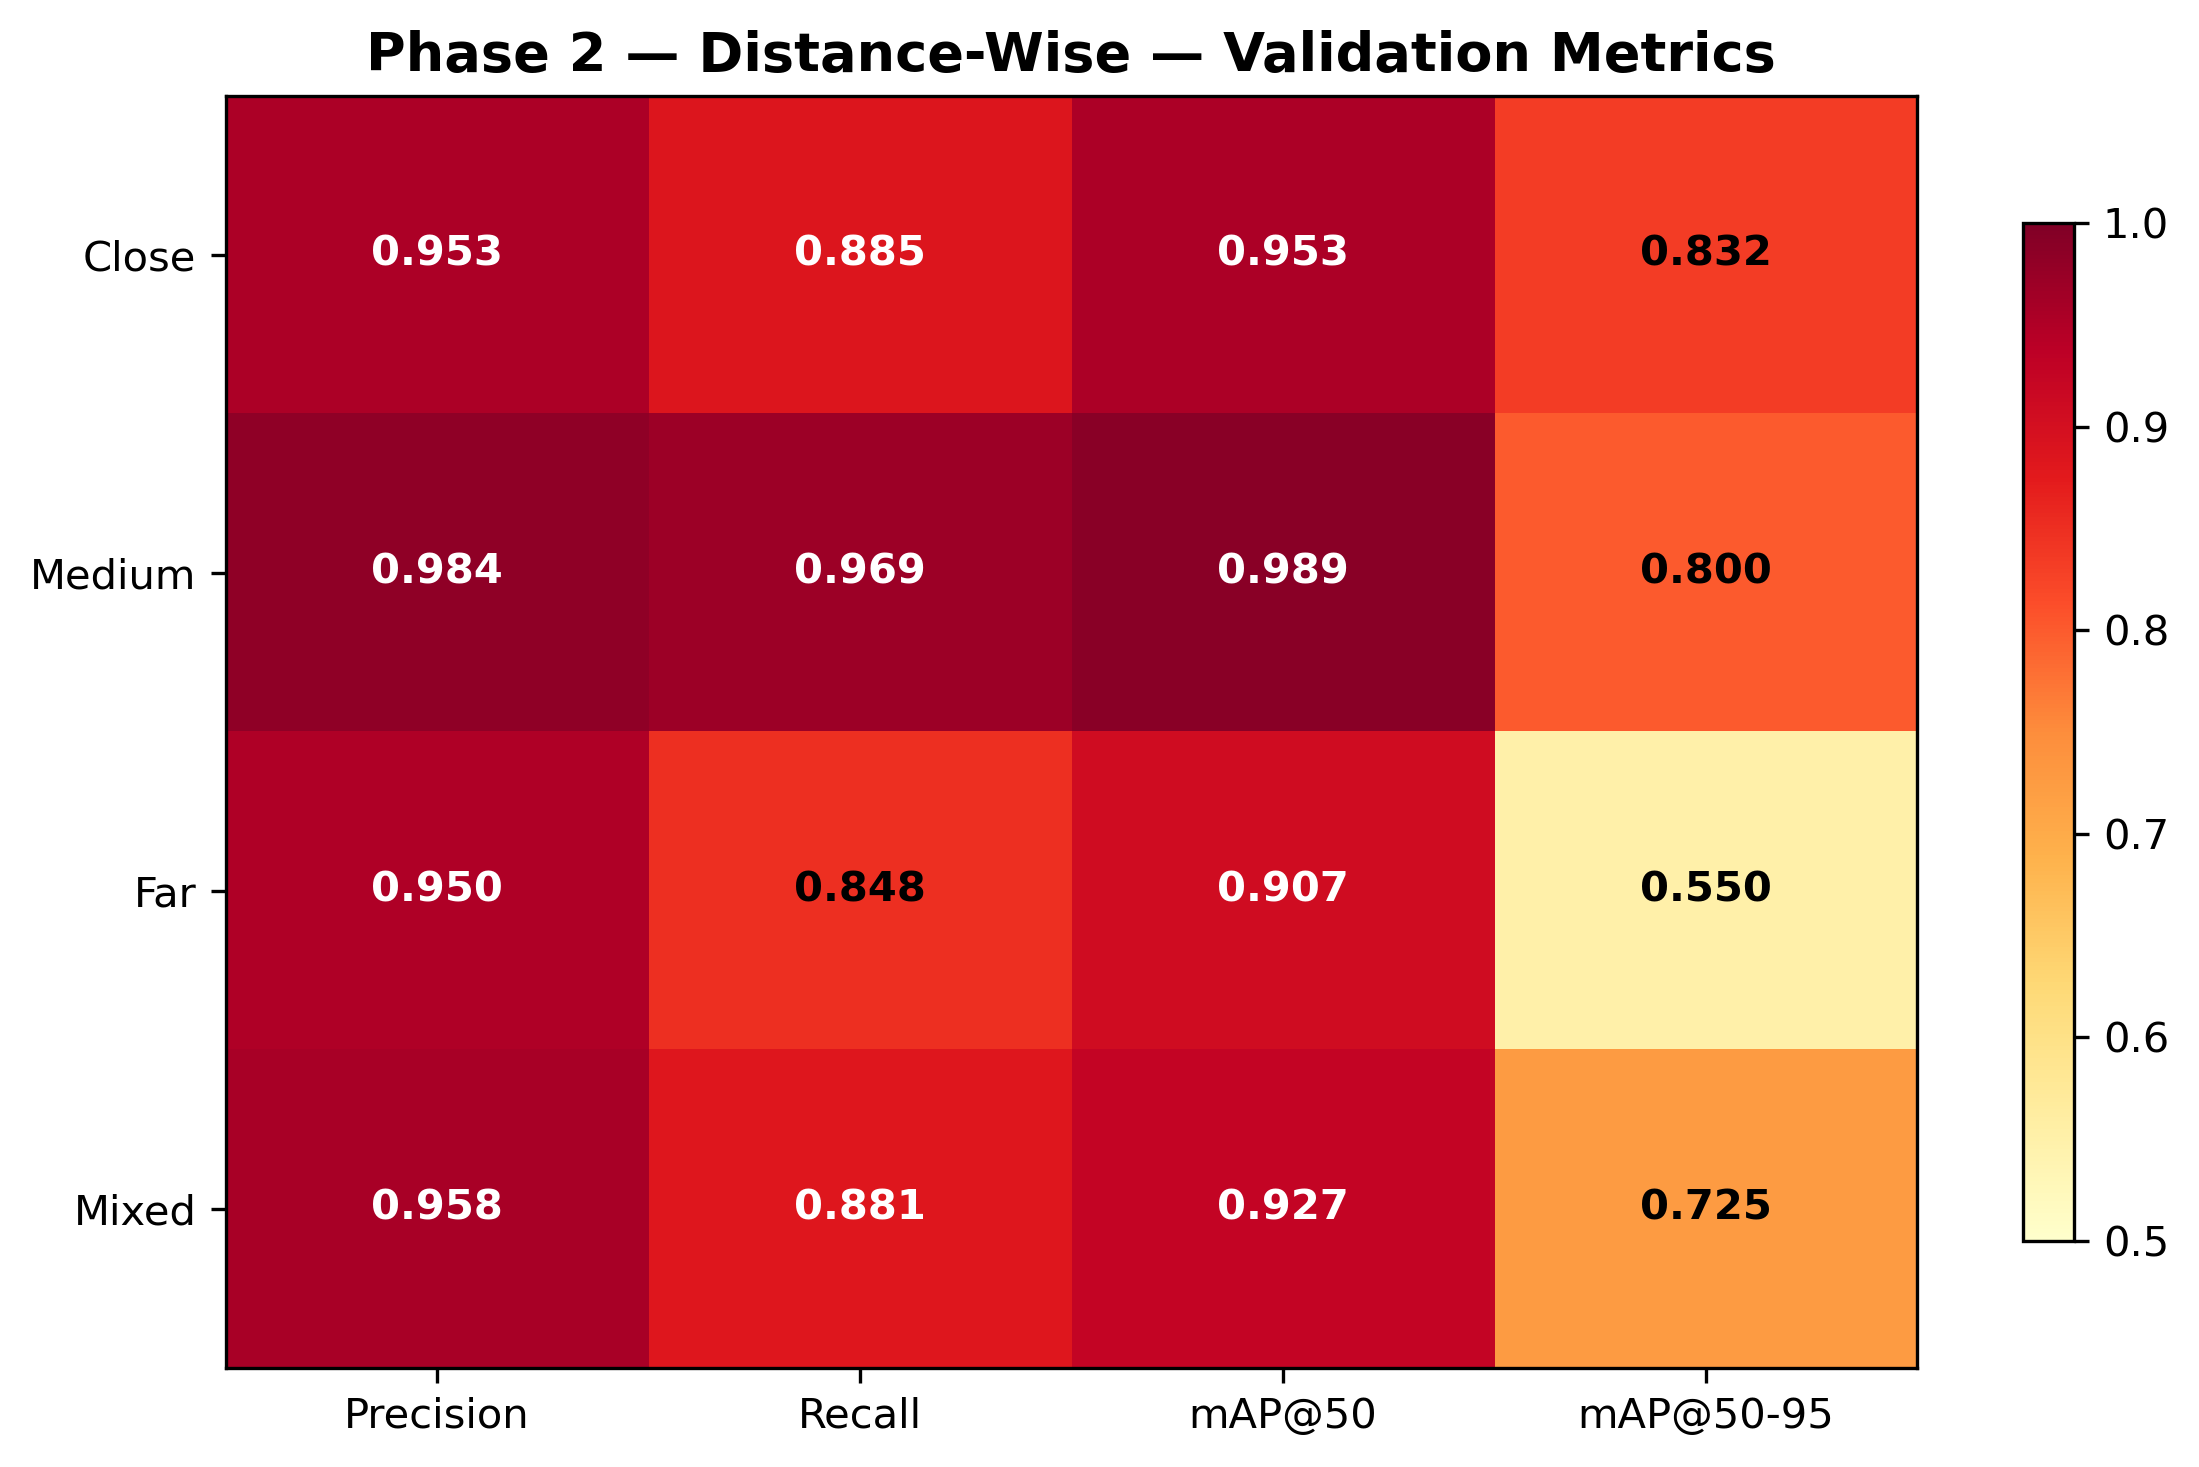
\includegraphics[width=0.78\textwidth]{graphs/distance_heatmap_phase2.png}
\caption{Heatmap of all distance-wise metrics after Phase~2.}
\label{fig:dist-heatmap}
\end{figure}

\textbf{What we can read from these numbers:}
\begin{itemize}[noitemsep]
    \item \textbf{Long-range} drones see the largest improvement in mAP@50
          ($0.8784 \rightarrow 0.9066$, $+3.21\%$). This is the hardest
          subset, and it is also the one that benefits most from the extra
          training in Phase~2.
    \item \textbf{Mid-range} reaches the best overall numbers
          ($\text{mAP@50} = 0.9889$ after Phase~2), which is what one would
          expect since these objects are large enough to be detected easily
          and small enough to fit nicely in the receptive field.
    \item \textbf{Close-range} shows a small drop in mAP@50 in Phase~2.
          Looking at it together with the other subsets, this seems to be the
          model giving up a little close-range specialisation in exchange for
          better generalisation everywhere else.
\end{itemize}

% --------------------------------------------------
\section{Environment-Wise Results}
\label{sec:env-results}

The same trained model was also validated on the three environment subsets
defined in Section~\ref{sec:env-split}.

\begin{table}[H]
\centering
\caption{Environment-wise validation -- Phase~1 (epoch 200).}
\label{tab:env-phase1}
\begin{tabular}{lcccc}
\toprule
\textbf{Environment}                & \textbf{P} & \textbf{R} & \textbf{mAP@50} & \textbf{mAP@50\,--\,95} \\
\midrule
Clear-sky   (bright clear)          & 0.9542 & 0.8890 & 0.9310 & 0.7141 \\
Low-light   (night / low-light)     & 0.9519 & 0.8710 & 0.9461 & 0.6246 \\
Cluttered                           & 0.9367 & 0.8487 & 0.9050 & 0.5952 \\
\bottomrule
\end{tabular}
\end{table}

\begin{table}[H]
\centering
\caption{Environment-wise validation -- Phase~2 (epoch 500).}
\label{tab:env-phase2}
\begin{tabular}{lcccc}
\toprule
\textbf{Environment}                & \textbf{P} & \textbf{R} & \textbf{mAP@50} & \textbf{mAP@50\,--\,95} \\
\midrule
Clear-sky   (bright clear)          & 0.9664 & 0.8943 & 0.9486 & 0.7331 \\
Low-light   (night / low-light)     & \textbf{0.9695} & 0.8840 & \textbf{0.9600} & 0.6583 \\
Cluttered                           & 0.9527 & 0.8425 & 0.9134 & 0.6087 \\
\bottomrule
\end{tabular}
\end{table}

\begin{figure}[H]
\centering
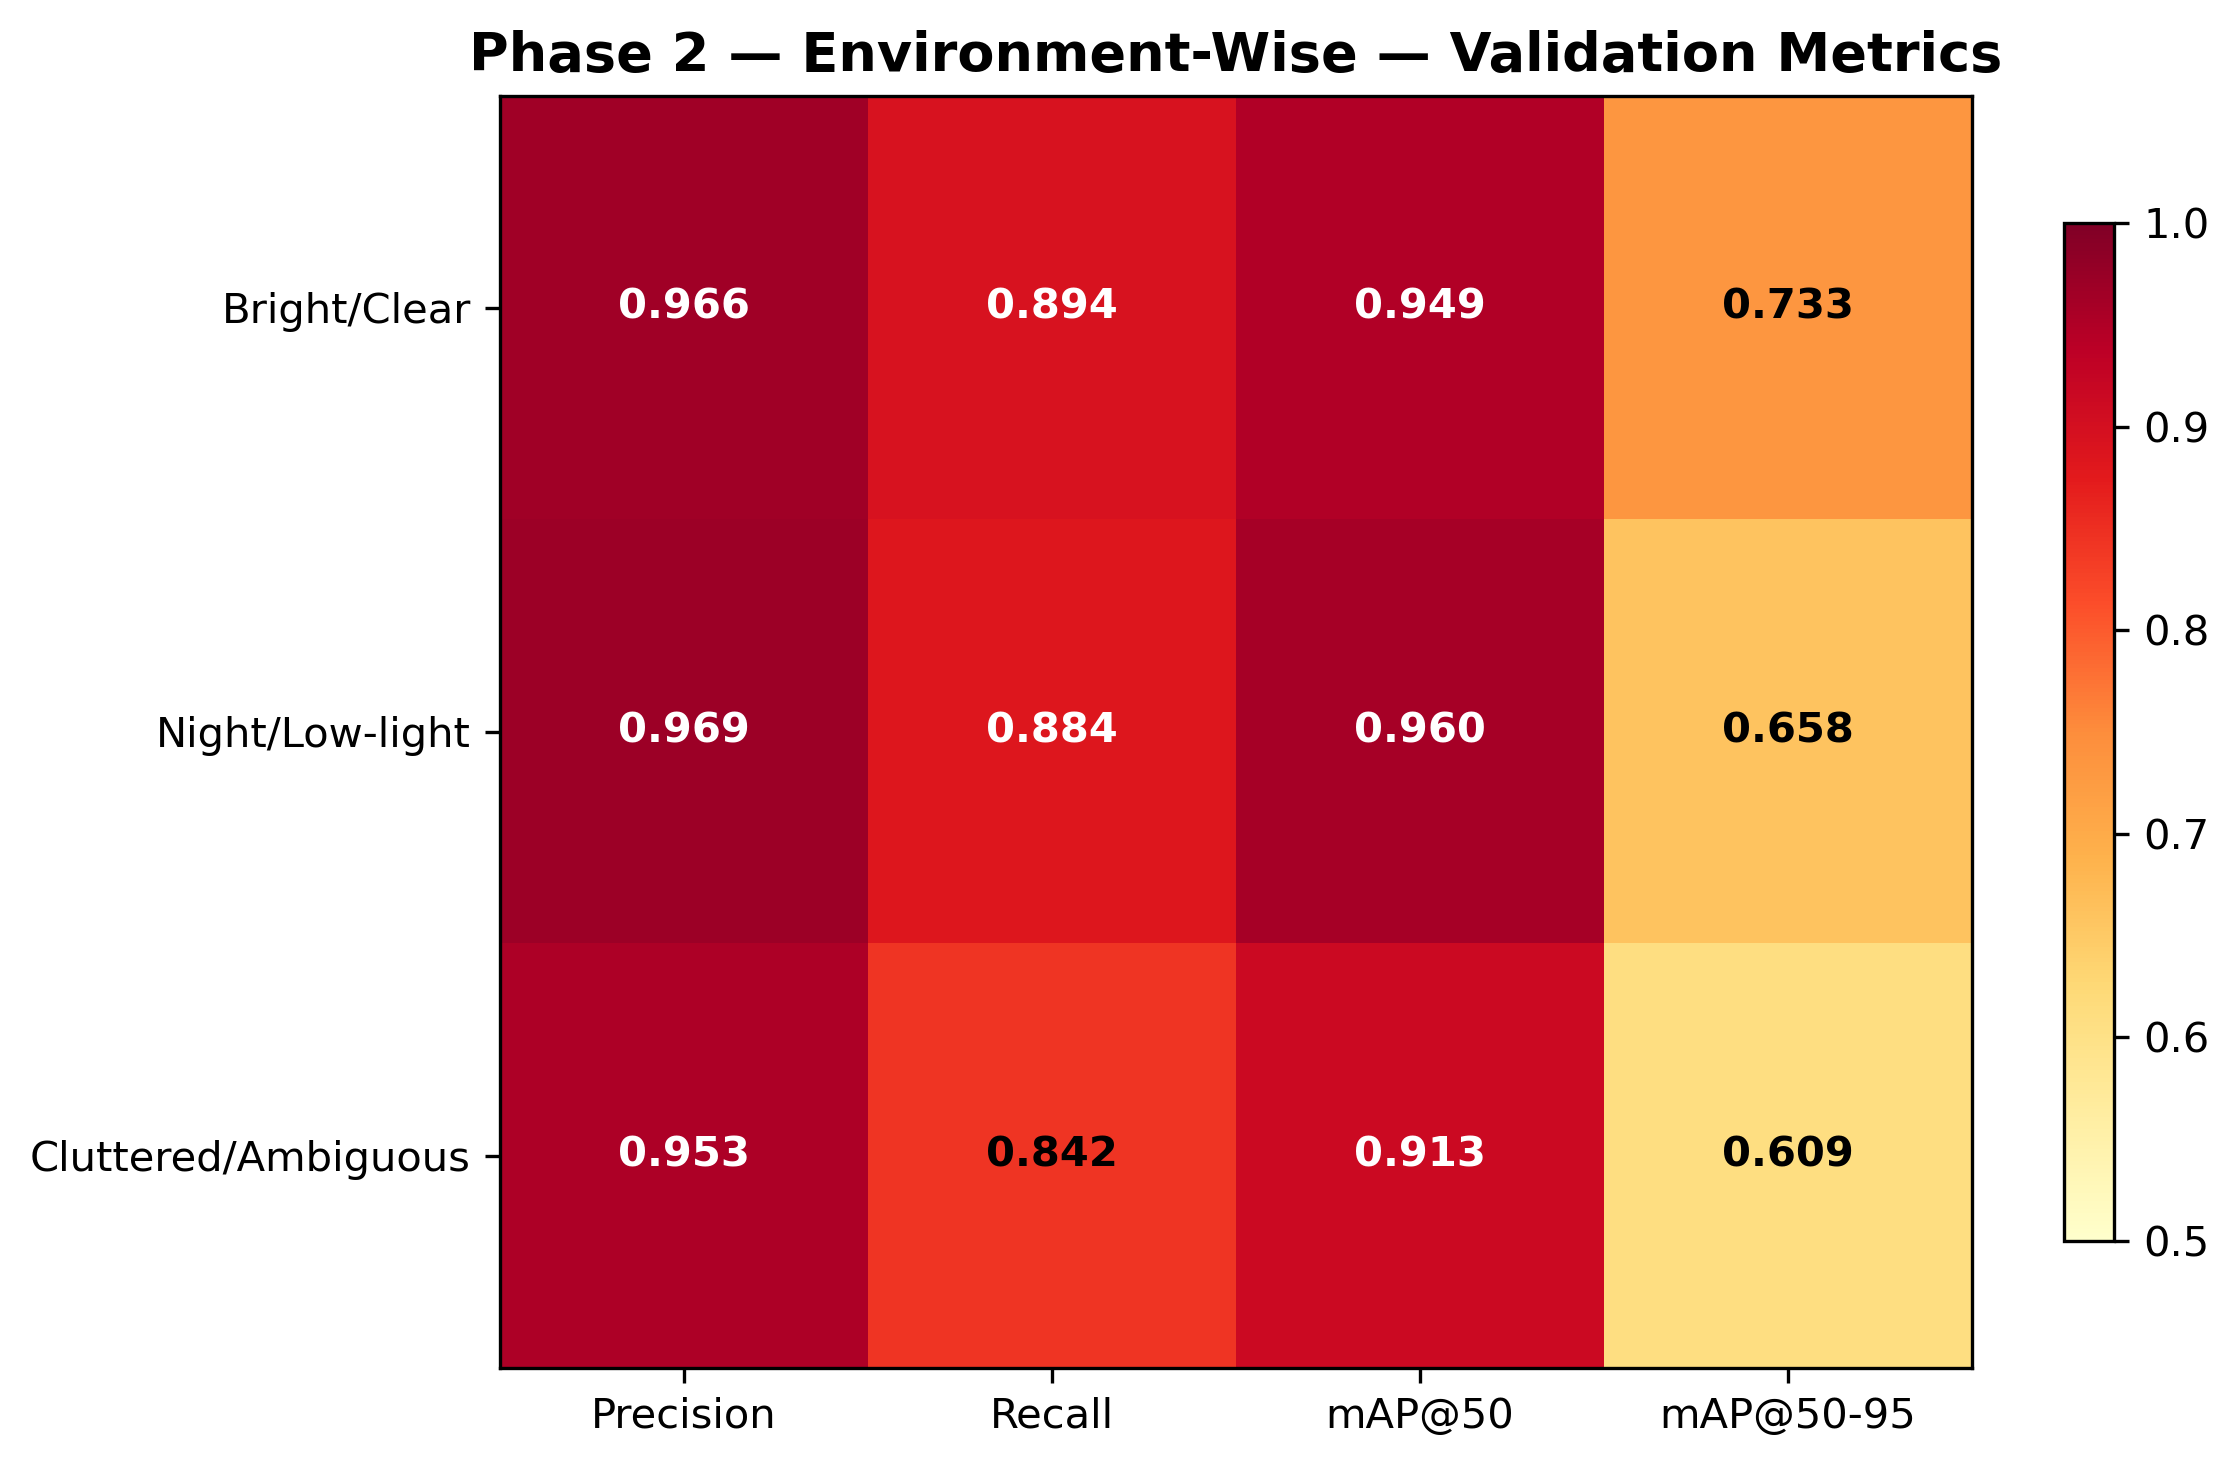
\includegraphics[width=0.78\textwidth]{graphs/environment_heatmap_phase2.png}
\caption{Heatmap of all environment-wise metrics after Phase~2.}
\label{fig:env-heatmap}
\end{figure}

\vspace{2cm}
\textbf{What we can read from these numbers:}
\begin{itemize}[noitemsep]
    \item All three environments improve in Phase~2 in precision, mAP@50 and
          mAP@50\,--\,95.
    \item \textbf{Low-light} sees the largest mAP@50\,--\,95 gain ($+5.40\%$)
          and the highest mAP@50 in Phase~2 ($0.9600$). This is a bit
          surprising at first, but on closer inspection it makes sense -- the
          drones in those images often carry small lights or contrast strongly
          with the dark background, which makes them easier to localise.
    \item \textbf{Cluttered} remains the hardest environment, which is what
          we expected: complex backgrounds produce more false positives.
\end{itemize}

% --------------------------------------------------
\section{Comparison with the existing YOLOv9 + EfficientNet-B3 Model}
\label{sec:vs-prior}

The earlier in-house pipeline was \textbf{YOLOv9 + EfficientNet-B3}, trained
on exactly the same drone/non-drone dataset. So the comparison below is done on the same data with the same
metric definitions wherever possible.

\subsection{Overall training and validation comparison}
Table~\ref{tab:vs-prior-train} compares the final training/validation
numbers reported at the end of the existing model training against our YOLO11-nano model. All loss values are the standard Ultralytics training losses
(box loss, classification loss, Distribution Focal Loss).

\begin{table}[H]
\centering
\caption{Overall comparison of the two pipelines on the same validation set.}
\label{tab:vs-prior-train}
\small
\setlength{\tabcolsep}{4pt}
\begin{tabular}{lcc}
\toprule
\textbf{Metric} & \textbf{YOLOv9 + EfficientNet-B3} & \textbf{This work: YOLO11-nano} \\
                & \textbf{(epoch 20, final)}                & \textbf{(Phase~2, epoch 500)} \\
\midrule
Precision               & 0.9383 & \textbf{0.9622} \\
Recall                  & \textbf{0.8953} & 0.8662 \\
mAP@50                  & 0.9307 & 0.9305 \\
mAP@50\,--\,95          & 0.6214 & \textbf{0.6727} \\
\midrule
Box loss (train)        & 0.9760 & \textbf{0.7614} \\
Classification loss     & 0.6431 & \textbf{0.3774} \\
DFL loss                & 1.2123 & \textbf{0.8826} \\
\bottomrule
\end{tabular}
\end{table}

The two pipelines reach almost the same mAP@50, but our YOLO11-nano model
gives a clearly better \textbf{precision} ($+2.4$ points) and a clearly
better \textbf{mAP@50\,--\,95} ($+5.1$ points), which means it draws tighter,
better-localised boxes around the drones. All three training losses are
also lower for YOLO11-nano, which is consistent with the longer training schedule.

\subsection{Distance-wise comparison}
The existing model's evaluation script reports a \emph{confidence score range} for
each distance category instead of full Precision/Recall/mAP numbers. The
confidence score is the model's own probability that the predicted box
contains a drone -- a higher value means the model is more sure about its
detections, but it does not directly tell us whether those detections are
correct. To make the comparison meaningful, we put the confidence
ranges next to the mAP@50 values that our model achieves on the same
distance subsets (Section~\ref{sec:dist-results}).

\begin{table}[H]
\centering
\caption{Distance-wise comparison.}
\label{tab:vs-prior-dist}
\small
\setlength{\tabcolsep}{4pt}
\begin{tabular}{lcc}
\toprule
\textbf{Distance subset} & \textbf{Existing model (confidence)} & \textbf{This work (mAP@50)} \\
\midrule
Close-range              & 0.93 -- 1.00 & 0.9534 \\
Mid-range                & 0.90 -- 0.96 & \textbf{0.9889} \\
Long-range (very far)    & 0.70 -- 0.78 & \textbf{0.9066} \\
\bottomrule
\end{tabular}
\end{table}

Both pipelines do well on close-range drones, where the target fills a
large part of the frame. The most important difference is on the
\textbf{long-range} subset: the existing model is clearly less confident on
distant drones (0.70--0.78), while YOLO11-nano still reaches an mAP@50 of
$0.9066$ on the same images. This matches what we expect from the
architecture -- the C2PSA attention block in YOLO11 is specifically
designed to help with small, distant targets.

\subsection{Environment-wise comparison}
The same kind of comparison is done for the three environment categories
defined in Section~\ref{sec:env-split}.

\begin{table}[H]
\centering
\caption{Environment-wise comparison.}
\label{tab:vs-prior-env}
\small
\setlength{\tabcolsep}{4pt}
\begin{tabular}{lcc}
\toprule
\textbf{Environment}       & \textbf{Existing model (confidence)} & \textbf{This work (mAP@50)} \\
\midrule
Bright / clear sky         & $\sim$1.00     & 0.9486 \\
Night / low-light          & 0.85 -- 0.98   & \textbf{0.9600} \\
Cluttered                  & 0.70 -- 0.80   & \textbf{0.9134} \\
\bottomrule
\end{tabular}
\end{table}

In bright, clean-sky scenes both pipelines do very well -- the existing
model is even slightly more confident on average. The gap opens up again
in the harder settings: on \textbf{cluttered} backgrounds the existing
model's confidence drops to 0.70--0.80, while YOLO11-nano holds an mAP@50 of
$0.9134$, and on \textbf{low-light} images both models stay strong but
YOLO11-nano is more consistent.

\subsection{Summary}
Putting the three tables together, the proposed YOLO11-nano pipeline does
better on this dataset for a few clear reasons:
\begin{itemize}[noitemsep]
    \item \textbf{The architecture is better suited to small objects.} The
          C2PSA attention block explicitly focuses on small targets, which
          is exactly the drone-on-sky setting and is reflected in the much
          better long-range numbers.
    \item \textbf{We trained for much longer.} 500 epochs in two phases vs
          20 epochs gives lower training losses on every component (box,
          classification, DFL) and a noticeably better mAP@50\,--\,95.
    \item \textbf{We evaluated more thoroughly.} The distance-wise and
          environment-wise splits give a much clearer picture of where each
          model is strong and where it is weak than a single mAP score
          would.
    \item \textbf{The model is lighter.} \texttt{yolo11n} has fewer
          parameters than YOLOv9~+~EfficientNet-B3, so the better numbers
          are obtained at a lower compute cost -- which matters for any
          future edge-deployment.
\end{itemize}

% =====================================================================
%  CHAPTER 5 — CONCLUSION AND FUTURE WORK
% =====================================================================
\chapter{Conclusion and Future Work}
\label{ch:conclusion}

\section{Conclusion}
This project picked YOLO11-nano out of six candidate detectors (YOLOv9, YOLO11,
RT-DETR, YOLO26, NSSRD, ED-Net), trained it on the in-house drone/non-drone
dataset that was originally built by Madhubani Basu, and evaluated it carefully
using overall validation, a distance-wise split, and an environment-wise split.

The final YOLO11-nano model reaches
\begin{center}
\textbf{P\,=\,0.9622, \; R\,=\,0.8662, \; mAP@50\,=\,0.9305,
\; mAP@50\,--\,95\,=\,0.6727}
\end{center}
on the full validation set, which is an improvement over the earlier existing
YOLOv9~+~EfficientNet-B3 result on the same data
(Section~\ref{sec:vs-prior}), and the model achieves this with fewer
parameters. The detailed per-subset results show that the model is robust
across distances and environments, with the largest gains from the extended
Phase~2 training observed for long-range drones and low-light scenes.

\section{Future Work}
\begin{enumerate}[noitemsep]
    \item \textbf{Higher input resolution.} Increasing the input from
          $320\times320$ to $640\times640$ should further help with the
          smallest, most distant drones, which are still the weakest subset.
    \item \textbf{Stronger augmentation.} Mosaic, mixup and adaptive
          augmentation policies, especially aimed at the cluttered subset,
          should reduce the false-positive rate in busy backgrounds.
    \item \textbf{Bigger and more diverse dataset.} Adding more images of
          drones in rain, fog and snow, and including a wider variety of
          drone shapes, would make the model more robust to real-world
          conditions that are not well represented in the current data.
    \item \textbf{Try a slightly larger YOLO11 variant.} Training
          \texttt{yolo11s} or \texttt{yolo11m} on the same data and comparing
          the results would tell us how much accuracy is being left on the
          table by sticking to the smallest variant.
    \item \textbf{Reduce false positives on bird-like objects.} Adding hard
          negative examples such as birds, kites and balloons during training
          would directly attack the most common confusion in real drone
          feeds.
\end{enumerate}

% =====================================================================
%  REFERENCES
% =====================================================================
\chapter*{References}
\addcontentsline{toc}{chapter}{References}
\begin{enumerate}[noitemsep]
    \item J.~Redmon, S.~Divvala, R.~Girshick, and A.~Farhadi, ``You Only Look
          Once: Unified, Real-Time Object Detection,'' in \textit{Proc.\ IEEE
          CVPR}, 2016.
    \item C.-Y.~Wang, I.-H.~Yeh, and H.-Y.~M.~Liao, ``YOLOv9: Learning What
          You Want to Learn Using Programmable Gradient Information,''
          \textit{arXiv:2402.13616}, 2024.
    \item Ultralytics, ``YOLO11 documentation,''
          \url{https://docs.ultralytics.com/models/yolo11/}, 2024.
    \item Y.~Zhao \textit{et~al.}, ``DETRs Beat YOLOs on Real-time Object
          Detection (RT-DETR),'' \textit{arXiv:2304.08069}, 2023.
    \item M.~Tan and Q.~V.~Le, ``EfficientNet: Rethinking Model Scaling for
          Convolutional Neural Networks,'' in \textit{Proc.\ ICML}, 2019.
    \item T.-Y.~Lin \textit{et~al.}, ``Microsoft COCO: Common Objects in
          Context,'' in \textit{Proc.\ ECCV}, 2014.
    \item M.~Basu, ``Drone Detection Using YOLOv9 with EfficientNet-B3
          Backbone,'' B.Tech Project Report, IIIT Guwahati, 2025.
\end{enumerate}

\end{document}
